\chapter{Fehlerkorrigierende Codes}

\section{Einführung}

Stellen Sie sich vor, Sie feiern Ihren 18. Geburtstag und wollen ihren besten Freunden einige Fotos aus ihrer Kindheit zeigen. Die Fotos sind aber leider alle verpixelt und können nicht richtig angezeigt werden! Oder stellen Sie sich vor, sie wollen in einigen Jahren Bilder von ihrem Date anschauen, die Bilder auf ihrer Festplatte sind jedoch unleserlich. \textit{Bad luck}? Fast genau dies ist dem Profi-Fotografen Tony Northrup geschehen, als er den 18. Geburtstag seiner Tochter mit Fotos aus deren Kindheit feiern wollte: \href{https://www.youtube.com/watch?v=xvbnhCDfREk}{Video}.

Bei der Übertragung von Bits über das Internet können einzelne Bits spontan verändert oder gelöscht werden -- dies kann fatale Folgen haben! Bei spontaner Änderung von einem 1 zu einem 0 (oder umgekehrt) spricht man von sogenanntem \textit{bit rot}.

\section{Prüfbits}

Buchstaben können auf unterschiedliche Weise kodiert sein -- bei ASCII werden beispielsweise sieben Bits pro Zeichen verwendet:

\begin{table}[H]
    \centering
    \begin{tabular}{c|c}
        Buchstabe & Kodierung          \\\midrule\midrule
        A         & \texttt{010000001} \\\midrule
        B         & \texttt{010000010} \\\midrule
        C         & \texttt{010000011} \\\midrule
        $\cdots$  & $\cdots$
    \end{tabular}
\end{table}
Bei der Datenübertragung können aber einzelne Bits spontan von einem \texttt{1} zu einem \texttt{0} werden (oder umgekehrt). Was könnte getan werden, um dieser Gefahr vorzubeugen?

Ein erster, einfacher Ansatz bestünde darin, jedem Code noch ein weiteres Bit anzuhängen, so dass die Summe der Bits immer gerade ist:

\begin{table}[H]
    \centering
    \begin{tabular}{c|c}
        Buchstabe & Kodierung                                \\\midrule\midrule
        A         & \texttt{010000001\underline{\textbf{0}}} \\\midrule
        B         & \texttt{010000010\underline{\textbf{0}}} \\\midrule
        C         & \texttt{010000011\underline{\textbf{1}}} \\\midrule
        $\cdots$  & $\cdots$
    \end{tabular}
\end{table}

Wenn sich \textit{ein} Bit nun spontan verändert, wird der Code als fehlerhaft erkannt, da die Summe der Bits, welche den Wert \texttt{1} haben, nicht mehr gerade ist. Ein Computer könnte nun also anfordern, dass der Code nochmals geschickt wird.

Die Idee von Prüfziffern ist, dass jede Prüfziffer nach dem gleichen Prinzip berechnet ist. Stimmt bei einem erhaltenen Code die Formel mit der Prüfziffer nicht überein, wird der Code als fehlerhaft erkannt.
\begin{myexercise}
    Folgende Prüfziffern sind alle nach der gleichen Regel berechnet. Können Sie die Regel erkennen?
    \begin{itemize}
        \item 31\textbf{6}
        \item 1298\textbf{0}
        \item 3333574\textbf{2}
        \item 2\textbf{8}
        \item 10\textbf{9}
    \end{itemize}
    Was wäre die Kontrollziffer für die Zahl 4163?

    \begin{myanswer}
        \[3 + 1 + 6 = 10\]
        \[1 + 2 + 9 + 8 + 0 = 20\]
        \[3 + 3 + 3 + 3 + 5 + 7 + 4 + 2=30\]
        etc.
        Für die Zahl 4163: 4163\textbf{6}
    \end{myanswer}
\end{myexercise}

Ein EAN bezeichnet einen sogenannten European Article Number. Fast alle käuflich erhältlichen Waren auf dem Markt enthalten einen solchen Code, welcher aus 13 Ziffern besteht. Häufig wird er in Form eines Strichcodes dargestellt, wobei zwei Striche eine Ziffer darstellen, sowie 2 mal 2 Striche, die den Rand angeben (s. \cref{fig:ean}).

\begin{figure}[H]
    \centering
    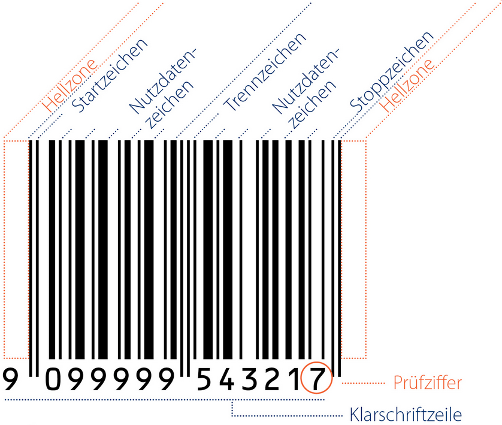
\includegraphics[width=0.7\linewidth]{GrundlagenInfo/05_ErrorChecking/Figures/EAN}
    \caption{Bestandteile eines EAN}
    \label{fig:ean}
\end{figure}

Ein EAN besteht aus 12 Ziffern und einer Prüfziffer:
\begin{equation}\label{eq:ean}
    x_1x_2x_3x_4x_5x_6x_7x_8x_9x_{10}x_{11}x_{12}\textcolor{red}{x_{13}}
\end{equation}


Das Scannen eines falschen Codes könnte zu falschen Preisen an der Kasse führen, weshalb EAN ebenfalls eine Prüfziffer enthalten, die sich wie folgt berechnet:

\begin{enumerate}
    \item $s=x_1+x_3+ x_5+ x_7+ x_9+ x_{11}+3\times( x_2+ x_4+ x_6+ x_8+ x_{10}+ x_{12})$
    \item Anschliessend wird $\textcolor{red}{x_{13}}$ so gewählt, dass $s+\textcolor{red}{x_{13}}$ durch 10 teilbar ist.
\end{enumerate}


\begin{myexercise}
    Welche folgender Fehler werden durch einen EAN erkannt?
    \begin{itemize}
        \item Vertippen (eine Ziffer ist falsch)
        \item Vertauschen zweier benachbarter Ziffern
        \item Auslassen (eine Ziffer wird vergessen)
        \item 2 mal Vertippen $\rightarrow$ 2 Ziffern werden falsch getippt
    \end{itemize}
\end{myexercise}

\begin{myexercise}
    Berechnen Sie für 978314221213 die EAN-13-Prüfziffer.
    \begin{myanswer}
        5
    \end{myanswer}
\end{myexercise}

\begin{myexercise}\label{ex:ean}
    Bestimmen Sie für den folgenden EAN-Code alle Paare von benachbarten Ziffern, deren Austausch in der Reihenfolge nicht erkannt werden kann:
    \begin{alltt}
        40\(\underset{\makebox[\widthof{\texttt{X}}][c]{\footnotesize\texttt{\red{3}}}}{\texttt{\red{3}}}\)05\(\underset{\makebox[\widthof{\texttt{X}}][c]{\footnotesize\texttt{\red{6}}}}{\texttt{\red{3}}}\)86\(\underset{\makebox[\widthof{\texttt{X}}][c]{\footnotesize\texttt{\red{9}}}}{\texttt{\red{5}}}\)74\(\underset{\makebox[\widthof{\texttt{X}}][c]{\footnotesize\texttt{\red{12}}}}{\texttt{\red{6}}}\)5
    \end{alltt}
    \begin{myanswer}
        Damit ein Austausch zweier benachbarter Ziffern nicht entdeckt würde, müsste sich die Summe $s$ um ein Vielfaches von 10 (oder 0) ändern. Dies wäre beispielsweise der Fall, wenn die zwei Ziffern 3 und 8 (Positionen 6 und 7) vertauscht würden.

        Der Beitrag der Ziffern zu $s$ im ursprünglichen und im abgeänderten Code sind in folgender Tabelle aufgelistet:


        \begin{table}[H]
            \centering
            \begin{tabular}{l|p{3cm}|p{4cm}|l}
                \textbf{Position} & \textbf{Ziffer} & \textbf{Gewichtung\newline (s. \cref{eq:ean})} & \textbf{Beitrag zu $s$} \\
                \midrule
                6                 & 3               & 3                                              & 9                       \\
                7                 & 8               & 1                                              & 8                       \\
            \end{tabular}
        \end{table}
        \[\Downarrow\]
        \begin{table}[H]
            \centering
            \begin{tabular}{l|p{3cm}|p{4cm}|l}
                \textbf{Position} & \textbf{Ziffer\newline (vertauscht)} & \textbf{Gewichtung\newline (s. \cref{eq:ean})} & \textbf{Beitrag zu $s$} \\
                \midrule
                6                 & 8                                    & 3                                              & 24                      \\
                7                 & 3                                    & 1                                              & 3                       \\
            \end{tabular}
        \end{table}

        Die Summe $s$ ändert sich also um:
        \[
            (24 + 3) - (9 + 8) = 27 - 17 = +10
        \]

        Da sich $s$ um ein Vielfaches von 10 verändert, bleibt die Prüfziffer gleich, und der Fehler wird nicht entdeckt.

        Dasselbe würde auch mit Positionen 5 und 6 funktionieren.
    \end{myanswer}

    \begin{mychallenge}
        Begründen Sie allgemein, für welche Arten von Ziffern ein Vertauschen zweier benachbarten Ziffern in einer EAN-Prüfziffer nicht entdeckt wird.
        \begin{myanswer}
            Damit ein Austausch zweier benachbarter Ziffern nicht entdeckt wird, darf sich die gewichtete Summe $s$ nicht ändern, da die Prüfziffer $x_{13}$ so gewählt ist, dass
            \[
                s + x_{13} \equiv 0 \mod 10
            \]
            gilt.

            Bezeichne die beiden benachbarten Ziffern mit $a$ und $b$ an den Positionen $i$ und $i+1$. Die zugehörigen Gewichte im EAN-System sind alternierend 1 und 3, also entweder $(g_i, g_{i+1}) = (1, 3)$ oder $(3, 1)$.

            Der ursprüngliche Beitrag dieser beiden Ziffern zur Summe $s$ ist:
            \[
                s_\text{alt} = g_i \cdot a + g_{i+1} \cdot b
            \]

            Nach dem Vertauschen lautet der Beitrag:
            \[
                s_\text{neu} = g_i \cdot b + g_{i+1} \cdot a
            \]

            Die Änderung der Summe beträgt also:
            \[
                \Delta s = s_\text{neu} - s_\text{alt} = g_i \cdot b + g_{i+1} \cdot a - (g_i \cdot a + g_{i+1} \cdot b)
                = (g_i - g_{i+1})(b - a)
            \]

            Da $g_i$ und $g_{i+1}$ abwechselnd $1$ und $3$ sind, ist $g_i - g_{i+1} \in \{-2, +2\}$. Es ergibt sich also:
            \[
                \Delta s = \pm 2 (b - a)
            \]

            Diese Änderung bleibt genau dann unbemerkt, wenn $\Delta s \equiv 0 \mod 10$ ist, also:
            \[
                \pm 2(b - a) \equiv 0 \mod 10 \quad \Leftrightarrow \quad b - a \equiv 0 \mod 5
            \]

            Es folgt:
            \[
                |b - a| \in \{0, 5\}
            \]

            Der Fall $b = a$ ist trivial, da keine Vertauschung erfolgt. Für eine echte Vertauschung mit $|b - a| = 5$ wird der Fehler \emph{nicht erkannt}.

            \medskip

            \textbf{Fazit:} Ein Vertauschen zweier benachbarter Ziffern im EAN-Code bleibt genau dann unentdeckt, wenn sich ihre Werte um 5 unterscheiden, also $|b - a| = 5$ gilt.

        \end{myanswer}
    \end{mychallenge}



\end{myexercise}

\begin{myexercise}
    Nehmen wir an, dass an der vierten Position im Code aus \cref{ex:ean} eine 8 statt der 0 getippt wurde. Finden Sie mindestens 5 Möglichkeiten, an anderen Stellen den Fehler so zu machen, dass die fehlerhafte Darstellung einem EAN-Code entspricht und somit dieser Doppelfehler unbemerkt bleibt.
    \begin{myanswer}
        Die Ziffer an Position 4 wurde von 0 auf 8 geändert. Da Position 4 das Gewicht 3 hat, verändert sich die Summe $s$ um
        \[
            (8-0) \cdot 3 = -24
        \]
        Damit der Doppelfehler unbemerkt bleibt, muss an einer anderen Stelle ein Fehler mit dem Beitrag $-24$, $-14$, $-4$, $+6$, $+16$ etc. gemacht werden. In diesem Fall verändert sich $s$ um 0, +10, +20, +30 etc., sodass $x_{13}$ gleich bleibt.

        Dies könnte mit folgenden möglichen Änderungen erfolgen:
        \[
            \begin{tabular}{l|l|l|l||l}
                \textbf{Position} & \textbf{Gewicht} & \textbf{Änderung} & \textbf{Fehlerbeitrag} & \textbf{Gesamt-Fehler} \\
                \midrule\midrule
                1                 & 1                & 4 $\rightarrow$ 0 & $-4$                   & $24-4=20$              \\\midrule
                2                 & 3                & 0 $\rightarrow$ 2 & $+6$                   & $24+6=30$              \\\midrule
                3                 & 1                & 3 $\rightarrow$ 9 & $+6$                   & $24+6=30$              \\\midrule
                9                 & 1                & 5 $\rightarrow$ 1 & $-4$                   & $24-4=20$              \\\midrule
                10                & 3                & 7 $\rightarrow$ 9 & $+6$                   & $24+6=30$              \\
            \end{tabular}
        \]

        In all diesen Fällen bleibt die Prüfziffer $x_{13}$ unverändert, der Doppelfehler wird also nicht erkannt.

    \end{myanswer}
\end{myexercise}

\begin{myexercise}
    Die ursprünglichen ISBN-10-Codes zur eindeutigen Bezeichnung von Büchern bestanden aus 9 Ziffern und einem Prüfsymbol aus {0,1,2,3,4,5,6,7,8,9,X}, wobei X die Zahl 10 repräsentierte. Für die neun Ziffern $x_1$, $x_2$, $\cdots$, $x_9$, hat man das Prüfsymbol $x_{10}$ wie folgt bestimmt:
    \[10\times x_1+9\times x_2+8\times x_3\cdots+2\times x_9 + x_{10}\]
    ist ein Vielfaches von 11. Falls $x_{10} = 10$ ist das Prüfsymbol $X$.
    \begin{enumerate}
        \item Bestimmen Sie für die folgenden Symbolfolgen, welche ISBN-10-Codes sind und welche es nicht sind:
              \begin{itemize}
                  \item 020144124\textbf{1}
                  \item 270004302\textbf{X}
                  \item 809004048\textbf{9}
                  \item 010144124\textbf{X}
              \end{itemize}
        \item Die neunstellige Zahl eines Buches ist 354042278. Bestimmen Sie das Prüfsymbol des ISBN-10-Codes des Buches.
    \end{enumerate}
    \begin{myanswer}
        \textbf{a) Prüfung der Symbolfolgen}

        Zur Erinnerung: Ein ISBN-10-Code ist gültig, wenn die gewichtete Summe
        \[
            10x_1 + 9x_2 + 8x_3 + \cdots + 2x_9 + x_{10} \equiv 0 \mod 11
        \]
        ist.

        Aufgabe (a): Wenn wir diese Formel anwenden, finden wir heraus, dass alle ausser dem zweiten Code gültige ISBN-Codes sind.

        Aufgabe (b): $3*10+5*9+4*8+0*7+4*6+2*5+2*4+7*3+8*2=186 \rightarrow x_{10}=1$, da $187=11*17$.

    \end{myanswer}

\end{myexercise}

\section{Fehler erkennen und korrigieren}

Sie kennen Fehlererkennung bereits aus Ihrem Alltag: So beispielsweise bei der Rechtschreibprüfung in Word, die Ihnen das korrekte Wort vorschlägt (s. \cref{fig:word})

\begin{figure}[H]
    \centering
    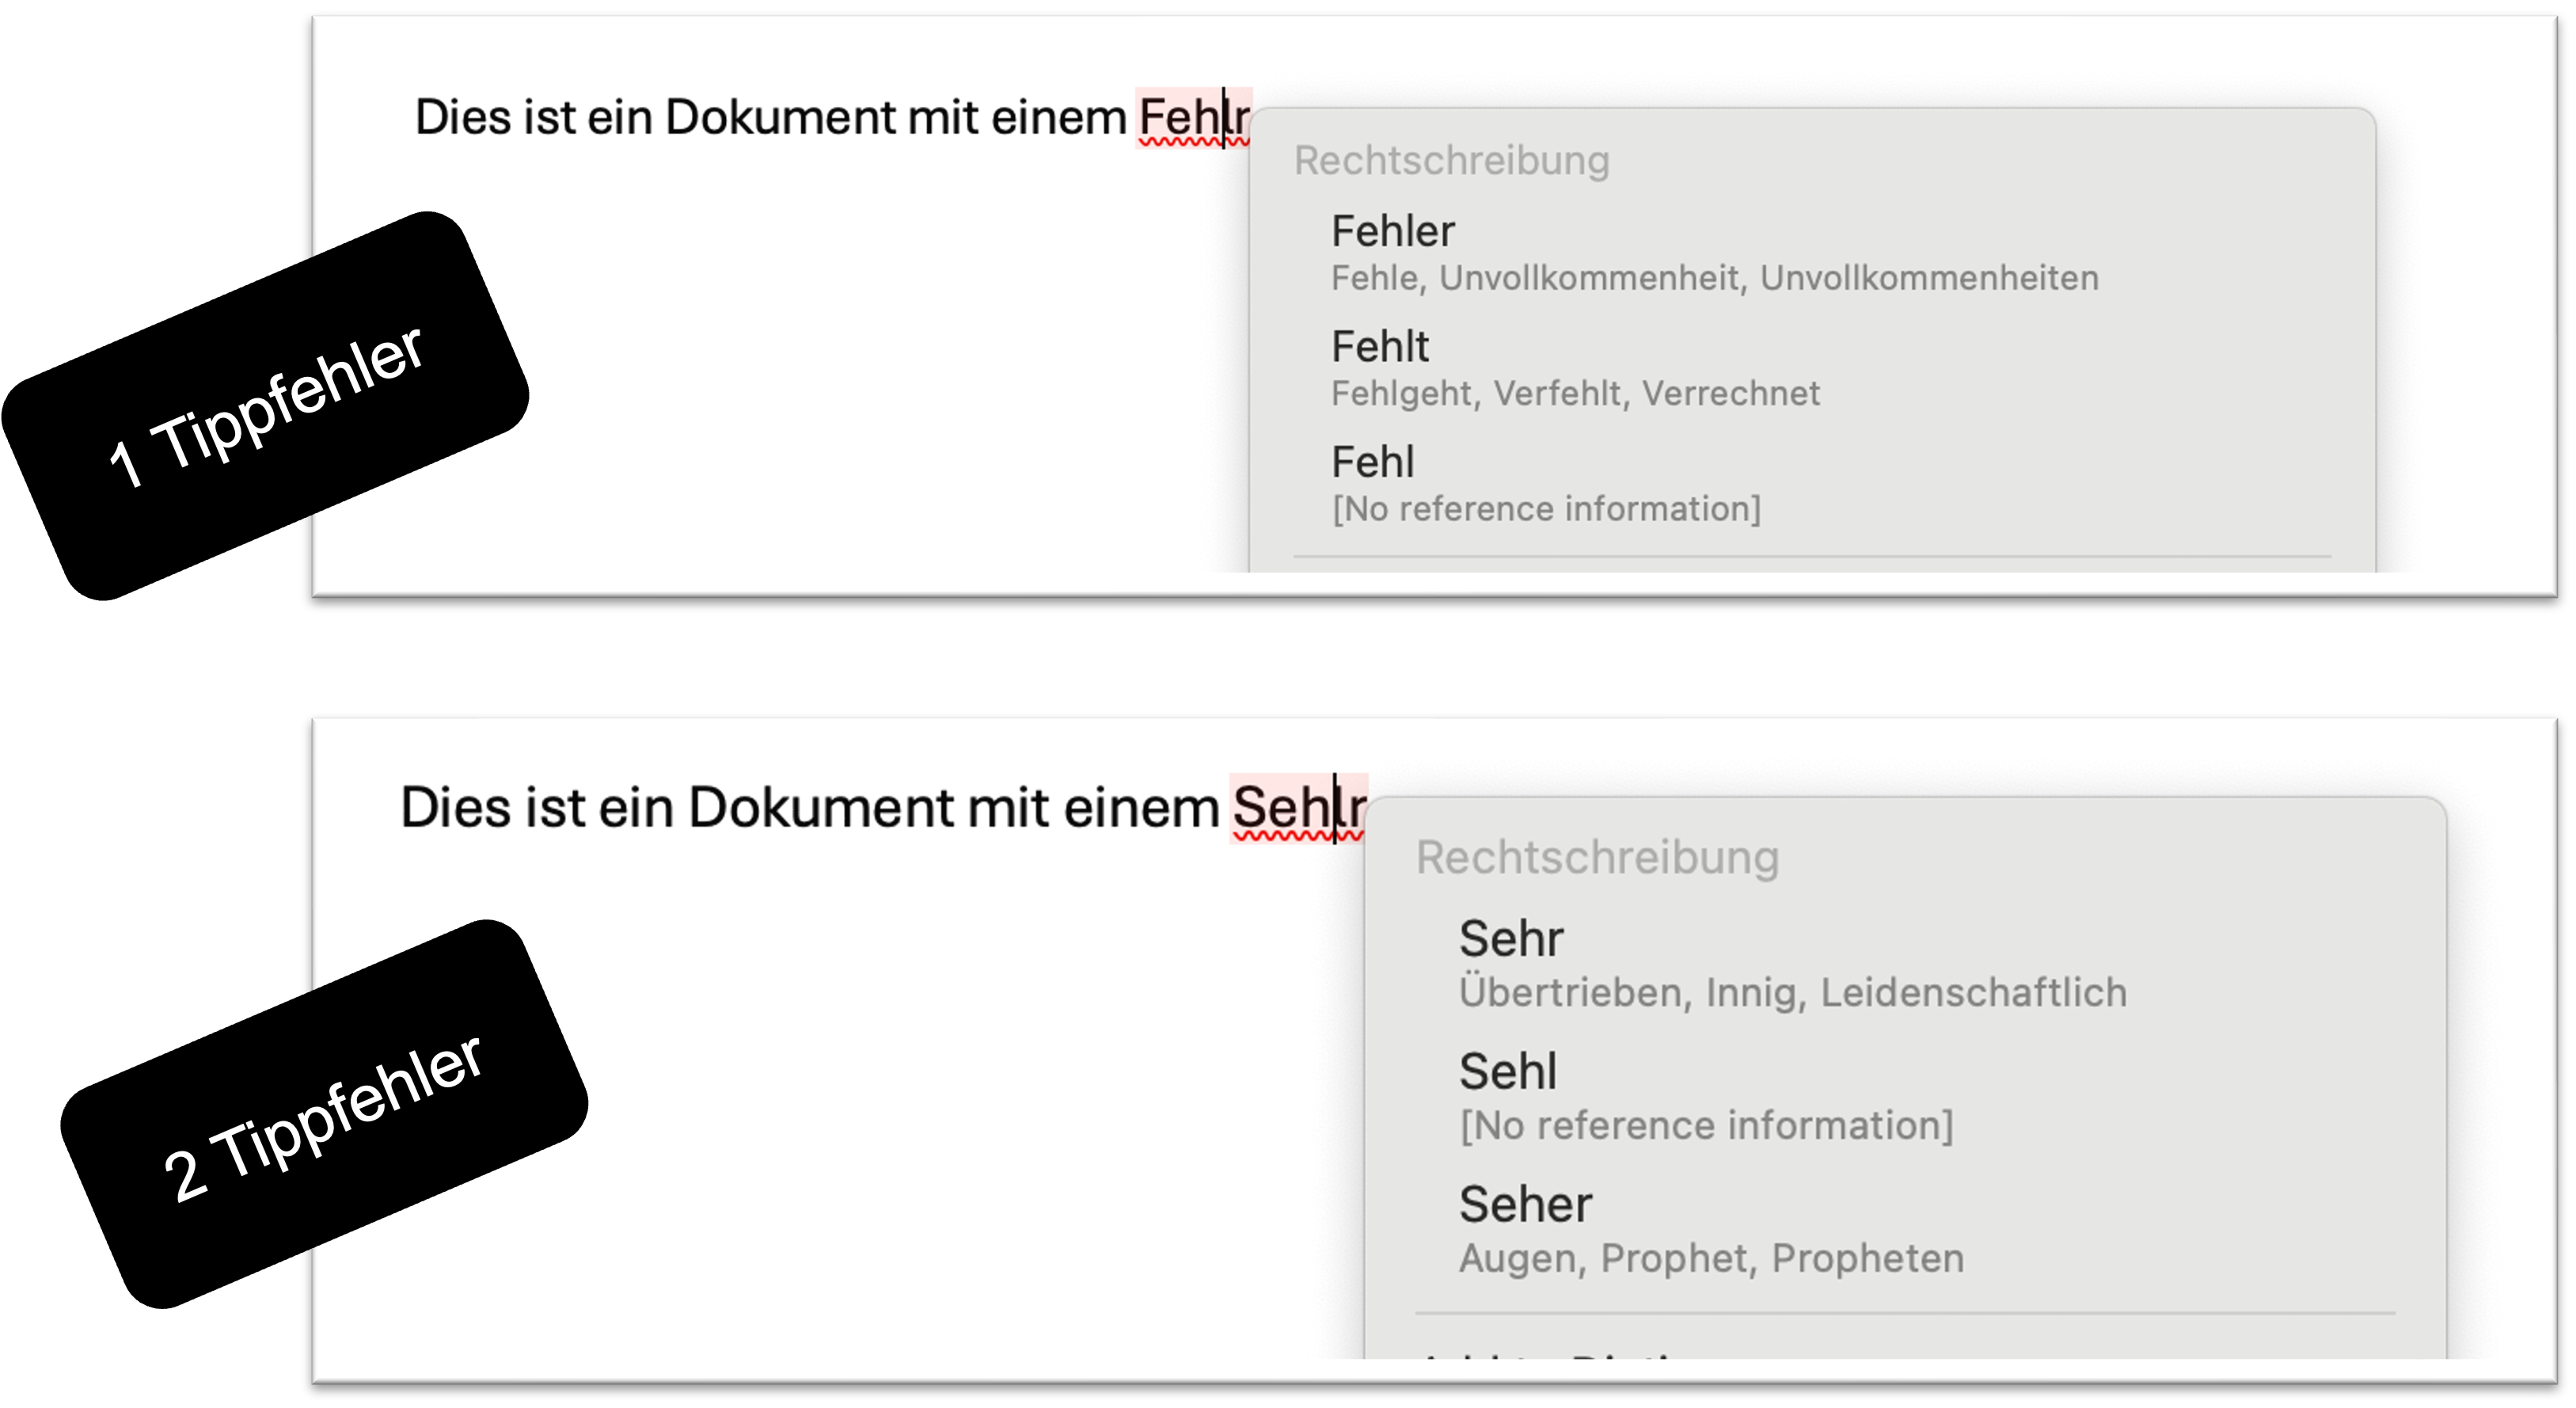
\includegraphics[width=0.7\linewidth]{GrundlagenInfo/05_ErrorChecking/Figures/Word}
    \caption{Rechtschreibprüfung im Programm Microsoft Word}
    \label{fig:word}
\end{figure}

\begin{myexample}\label{ex:word}
Wie viele Tippfehler werden im Beispiel aus \cref{fig:word} in jedem Fall erkannt?

Im gezeigten Beispiel wird ein Tippfehler noch erkannt. Es wird jedoch nicht jeder Tippfehler garantiert erkannt: So könnte beispielsweise ein Tippfehler vom ursprünglich gemeinten Wort \enquote{Fehler} hin zu \enquote{Zehler} nicht erkannt werden, da \enquote{Zehler} sowohl einen Buchstaben Abstand zum (korrekten, beabsichtigten) Wort \enquote{Fehler} wie auch zum (nicht beabsichtigten, aber korrekten) Wort \enquote{Zähler} hat.
\end{myexample}

Was können wir aus \cref{ex:word} lernen? Damit ein Fehler automatisch korrigiert werden kann, muss der Unterschied zwischen dem vertippten Wort und allen anderen möglichen Wörtern grösser sein als der Abstand zum ursprünglichen Wort.

Im Folgenden unterscheiden wir zwischen sogenannt \textbf{k-fehlererkennenden} und \textbf{k-fehlerkorrigierenden} Kodierungen. Eine Kodierung heisst \textbf{k-fehlererkennend}, wenn das Umflippen von 1, 2, $\cdots$ bis und mit \textbf{k} Bits in der Nachricht als Fehler erkannt wird. Falls bis zu \textbf{k} Fehler nicht nur erkannt sondern auch behoben werden können, spricht man von \textbf{k-fehlerkorrigierenden Kodierungen}.

\begin{myexample}\label{ex:code-kerk}
\cref{tab:codes} zeigt, wie eine Nachricht so kodiert werden kann, dass Fehler erkannt werden:
\begin{itemize}
    \item In Kodierung 1 handelt es sich schlicht und einfach um die ursprüngliche Nachricht.
    \item In Kodierung 2 wird die ursprüngliche Nachricht verdreifacht.
    \item In Kodierung 3 wird die ursprüngliche Nachricht verdoppelt, dazu kommt ein \textbf{Paritätsbit} (\underline{unterstrichen}) am Ende der Nachricht.
\end{itemize}
\begin{table}[H]
    \centering
    \begin{tabular}{c|c|c|c}
                         & \textbf{Kodierung$_1$} & \textbf{Kodierung$_2$}     & \textbf{Kodierung$_3$}                \\
        \midrule\midrule
        \textbf{Weiss}   & 00                     & 00\textcolor{orange}{0000} & 00\textcolor{orange}{00\underline{0}} \\
        \midrule
        \textbf{Gelb}    & 01                     & 01\textcolor{orange}{0101} & 01\textcolor{orange}{01\underline{1}} \\
        \midrule
        \textbf{Blau}    & 10                     & 10\textcolor{orange}{1010} & 10\textcolor{orange}{10\underline{1}} \\
        \midrule
        \textbf{Schwarz} & 11                     & 11\textcolor{orange}{1111} & 11\textcolor{orange}{11\underline{0}} \\
    \end{tabular}
    \caption{Kodierungstabelle}
    \label{tab:codes}
\end{table}

Wie viele Fehler werden durch die unterschiedlichen Kodierungen bestimmt erkannt?
\begin{itemize}
    \item In der ursprünglichen Kodierungen können Fehler nicht erkannt werden. Wird beispielsweise Weiss (\texttt{00}) fälschlicherweise als \texttt{01} versandt, geht der Empfänger davon aus, dass Gelb gesandt wurde und erkennt keine Fehler.
    \item In der zweiten Kodierung werden zwei Fehler erkannt, da es zwei \enquote{Mutationen} benötigt, um zu einem anderen Code zu werden.
    \item Bei der dritten Kodierung verhält es sich ebenso wie bei der zweiten.
\end{itemize}
Kodierung$_2$ und Kodierung$_3$ sind also betreffend Fehlererkennung gleich gut, allerdings ist Kodierung$_3$ kürzer und daher zu bevorzugen.
\end{myexample}

Um zu bestimmen, wie viele Fehler eine bestimmte Kodierung erkennen kann, müssen wir uns die Abstände zwischen allen möglichen Kode-Wörtern anschauen.

\begin{myexample}\label{ex:abstand}
Angenommen, wir hätten drei Code-Wörter, ANNA, ENZO und HANS, dann könnten die Abstände zwischen allen Code-Wörtern wie folgt bestimmt werden:

\begin{table}[H]
    \centering
    \begin{tabular}{c@{\hspace{1.5cm}}c@{\hspace{1.5cm}}c}
        \begin{tabular}{c}
            A N N A             \\
            \underline{E N Z O} \\
            x o x x             \\
            \textcolor{orange}{Abstand 3}
        \end{tabular}
         &
        \begin{tabular}{c}
            A N N A             \\
            \underline{H A N S} \\
            x x o x             \\
            \textcolor{orange}{Abstand 3}
        \end{tabular}
         &
        \begin{tabular}{c}
            E N Z O             \\
            \underline{H A N S} \\
            x x x x             \\
            \textcolor{orange}{Abstand 4}
        \end{tabular}
    \end{tabular}
    \caption{Abstände zwischen den Codewörtern ANNA, ENZO und HANS}
    \label{tab:hans}
\end{table}

Die \enquote{x} bezeichnen Stellen, an denen sich die Buchstaben unterscheiden und die \enquote{o} Stellen, an denen die Buchstaben gleich sind. Der Abstand zwischen einem Wort-Paar ergibt sich aus der Summe der \enquote{x}.

Der minimale Abstand in diesem Beispiel ist 3, daher könnten in dieser Kodierung bis zu 2 Fehler, bzw. \enquote{Mutationen} erkannt werden. ANNA $\rightarrow$ \textcolor{red}{A}N\textcolor{red}{Z}A würde als Fehler erkannt, ANNA $\rightarrow$ \textcolor{red}{E}N\textcolor{red}{ZO} jedoch nicht, da ENZO ein korrektes Kode-Wort ist.
\end{myexample}

Binär funktioniert die Abstandsbestimmung genau gleich wie in \cref{ex:abstand}.

\begin{myexample}\label{ex:bin}
Basierend auf Kodierung$_2$ aus \cref{tab:codes} könnten die Abstände zwischen allen Code-Wörtern wie folgt bestimmt werden:

\begin{table}[H]
    \centering
    \begin{tabular}{c@{\hspace{1.5cm}}c@{\hspace{1.5cm}}c}
        \begin{tabular}{c}
            \texttt{0 0 0 0 0 0 }            \\
            \texttt{\underline{0 1 0 1 0 1}} \\\
            o x o x o x                      \\
            \textcolor{orange}{Abstand 3}
        \end{tabular}
         &
        \begin{tabular}{c}
            \texttt{0 0 0 0 0 0 }            \\
            \texttt{\underline{1 0 1 0 1 0}} \\\
            x o x o x o                      \\
            \textcolor{orange}{Abstand 3}
        \end{tabular}
         &
        \begin{tabular}{c}
            \texttt{0 0 0 0 0 0 }            \\
            \texttt{\underline{1 1 1 1 1 1}} \\\
            x x x x x x                      \\
            \textcolor{orange}{Abstand 6}
        \end{tabular} \\
        \begin{tabular}{c}
            \texttt{0 1 0 1 0 1 }            \\
            \texttt{\underline{1 0 1 0 1 0}} \\\
            x x x x x x                      \\
            \textcolor{orange}{Abstand 6}
        \end{tabular}
         &
        \begin{tabular}{c}
            \texttt{0 1 0 1 0 1 }            \\
            \texttt{\underline{1 1 1 1 1 1}} \\\
            \texttt{x o x o x o }            \\
            \textcolor{orange}{Abstand 3}
        \end{tabular}
         &                                \\
        \begin{tabular}{c}
            \texttt{1 0 1 0 1 0 }            \\
            \texttt{\underline{1 1 1 1 1 1}} \\\
            \texttt{o x o x o x }            \\
            \textcolor{orange}{Abstand 3}
        \end{tabular}
         &
         &                                \\
    \end{tabular}
    \caption{Abstände zwischen allen Codewörtern der Kodierung$_2$ aus \cref{tab:codes}}
    \label{tab:abst-codes}
\end{table}

Damit können auch in diesem Beispiel bis zu 2 Fehler erkannt werden.
\end{myexample}

\begin{myexercise}\label{ex:xavier}
    Xavier schlägt vor, die Code-Wörter für die Farben aus \cref{ex:code-kerk} anders zu konstruieren. Man soll zu den Darstellungen (zwei Bits, z.B. 11) der Farben das Prüfbit anhängen (z.B. 11\underline{0}), sodass die Anzahl der Einsen gerade wird. Danach sollte man diese drei Bits in zwei Kopien (z.B. 11\underline{0}11\underline{0} für \enquote{Schwarz}) zu einem Code-Wort machen. Konstruieren Sie alle Code-Wörter der Kodierung und bestimmen Sie, wie viele Fehler man damit erkennen kann.
    \begin{myanswer}
        \begin{table}[H]
            \centering
            \begin{tabular}{c@{\hspace{1.5cm}}c@{\hspace{1.5cm}}c}
                \begin{tabular}{c}
                    \texttt{0 0 0 0 0 0 }            \\
                    \texttt{\underline{0 1 1 0 1 1}} \\\
                    \texttt{o x x o x x }            \\
                    \textcolor{orange}{Abstand 4}
                \end{tabular}
                 &
                \begin{tabular}{c}
                    \texttt{0 0 0 0 0 0 }            \\
                    \texttt{\underline{1 0 1 1 0 1}} \\\
                    \texttt{x o x x o x }            \\
                    \textcolor{orange}{Abstand 4}
                \end{tabular}
                 &
                \begin{tabular}{c}
                    \texttt{0 0 0 0 0 0 }            \\
                    \texttt{\underline{1 1 0 1 1 0}} \\\
                    \texttt{x x o x x o }            \\
                    \textcolor{orange}{Abstand 4}
                \end{tabular} \\
                \begin{tabular}{c}
                    \texttt{0 1 1 0 1 1 }            \\
                    \texttt{\underline{1 0 1 1 0 1}} \\\
                    \texttt{x x o x x o }            \\
                    \textcolor{orange}{Abstand 4}
                \end{tabular}
                 &
                \begin{tabular}{c}
                    \texttt{0 1 1 0 1 1 }            \\
                    \texttt{\underline{1 1 0 1 1 0}} \\\
                    \texttt{x o x x o x }            \\
                    \textcolor{orange}{Abstand 4}
                \end{tabular}
                 &                                \\
                \begin{tabular}{c}
                    \texttt{1 0 1 1 0 1 }            \\
                    \texttt{\underline{1 1 0 1 1 0}} \\\
                    \texttt{o x x o x x }            \\
                    \textcolor{orange}{Abstand 4}
                \end{tabular}
                 &
                 &                                \\
            \end{tabular}
            \caption{Abstände zwischen allen Codewörtern der Kodierung von Xavier}
            \label{tab:abst-codes-xavier}
        \end{table}
        Da der Mindestabstand zwischen allen Kodewörtern 4 ist, können bis zu 3 Fehler erkannt werden.
    \end{myanswer}
\end{myexercise}

\begin{myexercise}\label{ex:fehler-kodierungen}
    Bestimmen Sie, wie viele Fehler jede der folgenden Kodierungen erkennen kann. Bestimmen sie dazu als erstes den Mindest-Abstand innerhalb jeder Kodierung:
    \begin{table}[H]
        \centering
        \begin{tabular}{c|c|c|c|c}
                             & \textbf{4-Kopien} & \textbf{Xavier} & \textbf{1-Parity} & \textbf{0-Parity} \\
            \midrule\midrule
            \textbf{Weiss}   & \texttt{00000000} & \texttt{000000} & \texttt{000}      & \texttt{001}      \\
            \midrule
            \textbf{Gelb}    & \texttt{01010101} & \texttt{011011} & \texttt{011}      & \texttt{010}      \\
            \midrule
            \textbf{Blau}    & \texttt{10101010} & \texttt{101101} & \texttt{101}      & \texttt{100}      \\
            \midrule
            \textbf{Schwarz} & \texttt{11111111} & \texttt{110110} & \texttt{110}      & \texttt{111}      \\
        \end{tabular}
        \caption{Kodierungstabelle}
        \label{tab:kodierung}
    \end{table}
    \begin{myanswer}
        \begin{table}[H]
            \centering
            \begin{tabular}{c@{\hspace{1.5cm}}c@{\hspace{1.5cm}}c}
                \begin{tabular}{c}
                    \texttt{0 0 0 0 0 0 0 0}             \\
                    \texttt{\underline{0 1 0 1 0 1 0 1}} \\\
                    \texttt{o x o x o x o x }            \\
                    \textcolor{orange}{Abstand 4}
                \end{tabular}
                 &
                \begin{tabular}{c}
                    \texttt{0 0 0 0 0 0 0 0 }            \\
                    \texttt{\underline{1 0 1 0 1 0 1 0}} \\\
                    \texttt{x o x o x o x o }            \\
                    \textcolor{orange}{Abstand 4}
                \end{tabular}
                 &
                \begin{tabular}{c}
                    \texttt{0 0 0 0 0 0 0 0 }            \\
                    \texttt{\underline{1 1 1 1 1 1 1 1}} \\\
                    \texttt{x x x x x x x x }            \\
                    \textcolor{orange}{Abstand 8}
                \end{tabular} \\
                \begin{tabular}{c}
                    \texttt{0 1 0 1 0 1 0 1 }            \\
                    \texttt{\underline{1 0 1 0 1 0 1 0}} \\\
                    \texttt{x x x x x x x x }            \\
                    \textcolor{orange}{Abstand 8}
                \end{tabular}
                 &
                \begin{tabular}{c}
                    \texttt{0 1 0 1 0 1 0 1 }            \\
                    \texttt{\underline{1 1 1 1 1 1 1 1}} \\\
                    \texttt{x o x o x o x o }            \\
                    \textcolor{orange}{Abstand 4}
                \end{tabular}
                 &                                   \\
                \begin{tabular}{c}
                    \texttt{1 0 1 0 1 0 1 0 }            \\
                    \texttt{\underline{1 1 1 1 1 1 1 1}} \\\
                    \texttt{o x o x o x o x }            \\
                    \textcolor{orange}{Abstand 4}
                \end{tabular}
                 &
                 &                                   \\
            \end{tabular}
            \caption{Abstände zwischen allen Codewörtern der 4-Kopien-Kodierung}
            \label{tab:abst-4kopien}
        \end{table}
    \end{myanswer}
    \begin{myanswer}
        Kodierung von Xavier: s. Lösungen zu \cref{ex:xavier}.
    \end{myanswer}
    \begin{myanswer}
        \begin{table}[H]
            \centering
            \begin{tabular}{c@{\hspace{1.5cm}}c@{\hspace{1.5cm}}c}
                \begin{tabular}{c}
                    \texttt{0 0 0 }            \\
                    \texttt{\underline{0 1 1}} \\\
                    \texttt{o x x }            \\
                    \textcolor{orange}{Abstand 2}
                \end{tabular}
                 &
                \begin{tabular}{c}
                    \texttt{0 0 0 }            \\
                    \texttt{\underline{1 0 1}} \\\
                    \texttt{x o x }            \\
                    \textcolor{orange}{Abstand 2}
                \end{tabular}
                 &
                \begin{tabular}{c}
                    \texttt{0 0 0 }            \\
                    \texttt{\underline{1 1 0}} \\\
                    \texttt{x x o }            \\
                    \textcolor{orange}{Abstand 2}
                \end{tabular} \\
                \begin{tabular}{c}
                    \texttt{0 1 1 }            \\
                    \texttt{\underline{1 0 1}} \\\
                    \texttt{x x o }            \\
                    \textcolor{orange}{Abstand 2}
                \end{tabular}
                 &
                \begin{tabular}{c}
                    \texttt{0 1 1 }            \\
                    \texttt{\underline{1 1 0}} \\\
                    \texttt{x o x }            \\
                    \textcolor{orange}{Abstand 2}
                \end{tabular}
                 &                                \\
                \begin{tabular}{c}
                    \texttt{1 0 1 }            \\
                    \texttt{\underline{1 1 0}} \\\
                    \texttt{o x x }            \\
                    \textcolor{orange}{Abstand 2}
                \end{tabular}
                 &
                 &                                \\
            \end{tabular}
            \caption{Abstände zwischen allen Codewörtern der 1-Parity-Kodierung}
            \label{tab:abst-1parity}
        \end{table}
    \end{myanswer}
    \begin{myanswer}
        \begin{table}[H]
            \centering
            \begin{tabular}{c@{\hspace{1.5cm}}c@{\hspace{1.5cm}}c}
                \begin{tabular}{c}
                    \texttt{0 0 1 }            \\
                    \texttt{\underline{0 1 0}} \\\
                    \texttt{o x x }            \\
                    \textcolor{orange}{Abstand 2}
                \end{tabular}
                 &
                \begin{tabular}{c}
                    \texttt{0 0 1 }            \\
                    \texttt{\underline{1 0 0}} \\\
                    \texttt{x o x }            \\
                    \textcolor{orange}{Abstand 2}
                \end{tabular}
                 &
                \begin{tabular}{c}
                    \texttt{0 0 1 }            \\
                    \texttt{\underline{1 1 1}} \\\
                    \texttt{x x o }            \\
                    \textcolor{orange}{Abstand 2}
                \end{tabular} \\
                \begin{tabular}{c}
                    \texttt{0 1 0 }            \\
                    \texttt{\underline{1 0 0}} \\\
                    \texttt{x x o }            \\
                    \textcolor{orange}{Abstand 2}
                \end{tabular}
                 &
                \begin{tabular}{c}
                    \texttt{0 1 0 }            \\
                    \texttt{\underline{1 1 1}} \\\
                    \texttt{x o x }            \\
                    \textcolor{orange}{Abstand 2}
                \end{tabular}
                 &                                \\
                \begin{tabular}{c}
                    \texttt{1 0 0 }            \\
                    \texttt{\underline{1 1 1}} \\\
                    \texttt{o x x }            \\
                    \textcolor{orange}{Abstand 2}
                \end{tabular}
                 &
                 &                                \\
            \end{tabular}
            \caption{Abstände zwischen allen Codewörtern der 0-Parity-Kodierung}
            \label{tab:abst-0parity}
        \end{table}
    \end{myanswer}
    \begin{myanswer}
        Mindest-Abstände:
        \begin{itemize}
            \item 4-Kopien: 4
            \item Xavier: 4
            \item 1-Parity: 2
            \item 0-Parity: 2
        \end{itemize}
    \end{myanswer}
\end{myexercise}

\begin{mychallenge}\label{challenge:3code}
    Finden Sie eine binäre Kodierung mit 3 Code-Wörtern der Länge 5 und Mindest-Abstand 3.
\end{mychallenge}

\begin{mychallenge}
    Gibt es eine binäre Kodierung mit 3 Code-Wörtern der Länge 5 und Mindest-Abstand 3, welche die Code-Wörter 00000 und 11111 beinhaltet?
\end{mychallenge}



\section{Selbstkorrigierende Codes}

Bisher haben wir gelernt, Kodierungen für gewisse Nachrichten zu finden, so dass ein gewisser Mindestabstand gewährleistet wird. Durch einen Mindestabstand von 2 (Bits) zwischen jedem Nachrichtenpaar wird gewährleistet, dass ein Fehler bestimmt erkannt wird, da es zwei Fehler (ungewollte Bit-Änderungen) bräuchte, damit aus einem gültigen Codewort ein anderes, gültiges Codewort wird.

Falls wir einen Mindestabstand von 3 haben, können wir einen Fehler sogar \textit{korrigieren}: Bei einer einzigen Änderung eines Bits wäre das resultierende Codewort dann immer noch näher an am ursprünglichen Codewort als an allen anderen Codewörtern.

\begin{myexercise}\label{ex:fehlerkorrektur}
    Finden Sie für die drei Nachrichten Rot, Blau und Grün eine Kodierung aus Bitfolgen der Länge 5, die 1-fehlerkorrigierend ist.

    Das bedeutet, wenn ein Fehler vorkommt, weiss man nicht nur, dass die Nachricht fehlerhaft ist, sondern man kann das ursprüngliche Codewort aus der fehlerbehafteten Bitfolge eindeutig rekonstruieren. Was können Sie über den Abstand einer solchen Kodierung sagen?

    \begin{table}[H]
        \centering
        \begin{tabular}{c|c}
            \textbf{Farbe} & \textbf{Kodierung} \\\midrule\midrule
            Rot            & \texttt{00000}     \\\midrule
            Grün           &                    \\\midrule
            Blau           &                    \\
        \end{tabular}
    \end{table}
    \begin{myanswer}
        Mehrere Lösungen sind möglich, zum Beispiel:

        \begin{table}[H]
            \centering
            \begin{tabular}{c|c}
                \textbf{Farbe} & \textbf{Kodierung} \\\midrule\midrule
                Rot            & \texttt{00000}     \\\midrule
                Grün           & \texttt{00111}     \\\midrule
                Blau           & \texttt{11100}     \\
            \end{tabular}
        \end{table}
        Weshalb funktioniert die in diesem Beispiel dargestellte Kodierung, um einen Fehler zu korrigieren?

        Wir haben zwischen allen drei Kodierungen mindestens einen Abstand von 3:
        \begin{table}[H]
            \centering
            \begin{tabular}{c@{\hspace{1.5cm}}c@{\hspace{1.5cm}}c}
                \begin{tabular}{c}
                    \texttt{0 0 0 0 0}             \\
                    \texttt{\underline{0 0 0 1 1}} \\
                    \texttt{o o x x x}             \\
                    \textcolor{orange}{Abstand 3}
                \end{tabular}
                 &
                \begin{tabular}{c}
                    \texttt{0 0 0 0 0}             \\
                    \texttt{\underline{1 1 1 0 0}} \\
                    \texttt{x x x o o}             \\
                    \textcolor{orange}{Abstand 3}
                \end{tabular}
                 &
                \begin{tabular}{c}
                    \texttt{0 0 1 1 1}             \\
                    \texttt{\underline{1 1 1 0 0}} \\
                    \texttt{x x 0 x x}             \\
                    \textcolor{orange}{Abstand 4}
                \end{tabular}
            \end{tabular}
            \caption{Abstände zwischen allen Codewörtern der vorgeschlagenen Kodierung}
        \end{table}

        Angenommen, rot mutiert spontan zu folgendem Code:

        \texttt{0 0 0 0 0} $\rightarrow$ \texttt{0 0 0 \textcolor{red}{1} 0}

        Wir wissen, dass es sich bei \texttt{0 0 0 \textcolor{red}{1} 0} nicht um eine gültige Codefolge handelt. Die Abstände zu den gültigen Codefolgen sind:
        \begin{table}[H]
            \centering
            \begin{tabular}{c@{\hspace{1.5cm}}c@{\hspace{1.5cm}}c}
                \begin{tabular}{c}
                    \texttt{0 0 0 \textcolor{red}{1} 0} \\
                    \texttt{\underline{0 0 0 0 0}}      \\
                    \texttt{o o o x o}                  \\
                    \textcolor{orange}{Rot: Abstand 1}
                \end{tabular}
                 &
                \begin{tabular}{c}
                    \texttt{0 0 0 \textcolor{red}{1} 0} \\
                    \texttt{\underline{0 0 1 1 1}}      \\
                    \texttt{o o x o x}                  \\
                    \textcolor{orange}{Grün: Abstand 2}
                \end{tabular}
                 &
                \begin{tabular}{c}
                    \texttt{0 0 0 \textcolor{red}{1} 0} \\
                    \texttt{\underline{1 1 1 0 0}}      \\
                    \texttt{x x x x o}                  \\
                    \textcolor{orange}{Blau: Abstand 4}
                \end{tabular}
            \end{tabular}
            \caption{Abstände des mutierten Codes zu allen gültigen Codewörtern}
        \end{table}
        Es gibt nur ein Codewort, zu dem der Abstand am kürzesten ist: rot (Abstand 1). Daher muss es sich beim ursprünglichen Code um das Wort ``rot'' gehandelt haben und wir können den Code somit automatisch korrigieren, sofern wir wissen, dass genau ein Fehler passiert ist.
    \end{myanswer}
\end{myexercise}

\begin{mychallenge}\label{challenge:4bits}
    Könnte man \cref{ex:fehlerkorrektur} auch mit nur 4 Bits lösen?
\end{mychallenge}


In \cref{challenge:4bits} haben wir versucht, eine binäre Kodierung mit 4 Bits für 3 Nachrichten zu finden. Um die Aufgabe einfacher zu lösen, können wir uns ein Hilfsmittel zunutze machen. Dabei zeichnen wir alle möglichen Codes der Länge 4 auf und verbinden diejenigen Codes, welche Abstand 1 haben, miteinander (s. \cref{fig:4d}). Wenn wir nun einen Fehler korrigieren wollen, brauchen wir mindestens einen Abstand von 3 zwischen jedem benachbarten Bitpaar.

\begin{mydefinition}
Um die Anzahl möglicher 1-fehlerkorrigierender Codewörter für eine gewisse Code-Länge herauszufinden, gehen wir wie folgt vor:
\begin{enumerate}
    \item Wähle irgendein Codewort als erstes Codewort aus, z.B., \texttt{0000}.
    \item Streiche alle Code-Wörter, welche von allen bisher ausgewählten Codewörtern weniger als Abstand 3 entfernt sind, also alle Codewörter mit Abstand 1 oder 2.
    \item Wiederhole Schritte 1 und 2, bis alle Codewörter entweder ausgewählt oder durchgestrichen sind. Die Anzahl ausgewählte Codewörter bestimmt, wie viele Wörter wir kodieren können bei gleichzeitiger Garantie, immer bis zu einem Fehler korrigieren zu können.
\end{enumerate}
Soll der Code nur 1-fehlererkennend und nicht 1-fehlerkorrigierend sein, reicht es aus, in Schritt 2 alle Codewörter mit Abstand 1 zu streichen.

Dieses Vorgehen funktioniert auch für andere Code-Längen, beispielsweise 2 (\cref{fig:2d}), 3 (\cref{fig:3d}) oder 5 (\cref{fig:5d}).
\end{mydefinition}

\begin{figure}[H]
    \centering
    \begin{tikzpicture}
        \HyperCube{2}
    \end{tikzpicture}
    \caption{2D-Hyperwürfel}
    \label{fig:2d}
\end{figure}

\begin{figure}[H]
    \centering
    \begin{tikzpicture}
        \HyperCube{3}
    \end{tikzpicture}
    \caption{3D-Hyperwürfel}
    \label{fig:3d}
\end{figure}

\begin{figure}[H]
    \centering
    \begin{tikzpicture}
        \HyperCube{4}
    \end{tikzpicture}
    \caption{4D-Hyperwürfel}
    \label{fig:4d}
\end{figure}

\begin{figure}[H]
    \centering
    \resizebox{\textwidth}{!}{
        \begin{tikzpicture}
            \HyperCube{5}
        \end{tikzpicture}}
    \caption{5D-Hyperwürfel}
    \label{fig:5d}
\end{figure}

\begin{myexercise}
    Man verwendet eine Kodierung mit folgenden 4 Code-Wörtern der Länge 5:
    \begin{enumerate}[label=(\Alph*)]
        \item \texttt{00000}
        \item \texttt{00110}
        \item \texttt{11001}
        \item \texttt{11111}
    \end{enumerate}

    Bei welchen der folgenden Bitfolgen kann man eindeutig den Fehler korrigieren, falls man sicher ist, dass genau ein Fehler passiert ist?
    \begin{enumerate}
        \item \texttt{10000}
        \item \texttt{11101}
        \item \texttt{01111}
        \item \texttt{00100}
    \end{enumerate}

    \begin{myanswer}
        \begin{enumerate}
            \item \texttt{10000} -- ja: Abstand zu (A) kleiner als zu allen anderen gültigen Codewörtern
            \item \texttt{11101} -- nein: Abstand zu (C) und (D) gleich
            \item \texttt{01111} -- ja: Abstand zu (D) kleiner als zu allen anderen gültigen Codewörtern
            \item \texttt{00100} -- nein: Abstand zu (A) und (B) gleich
        \end{enumerate}

    \end{myanswer}
\end{myexercise}



\begin{myexercise}
    Zeichnen Sie alle \textbf{1-Fehler-erkennenden} Kodierungen im unten stehenden Hyperwürfel ein, ausgehend vom Code \texttt{011}. Wie viele Code-Wörter können Sie finden?
    \begin{figure}[H]
        \centering
        \begin{tikzpicture}
            \HyperCube{3}
        \end{tikzpicture}
        \caption{3D-Hyperwürfel}
    \end{figure}

    \begin{myanswer}

        \begin{figure}[H]
            \centering
            \begin{tikzpicture}
                \HyperCube{3}
                \CircleNodes{hg-011}

                % Cross out multiple nodes
                \CrossOutNodes{hg-001,hg-010,hg-111}
                \CircleNodes[green]{hg-101,hg-110,hg-000}
                \CrossOutNodes{hg-100}
            \end{tikzpicture}
            \caption{3D-Hyperwürfel}
        \end{figure}
        Vier gültige Codewörter: \texttt{011}, \texttt{101}, \texttt{000} und \texttt{110}
    \end{myanswer}

\end{myexercise}

\begin{myexercise}
    Zeichnen Sie alle \textbf{1-Fehler-korrigierenden} Kodierungen im unten stehenden Hyperwürfel ein, ausgehend vom Code \texttt{011}.
    \begin{figure}[H]
        \centering
        \begin{tikzpicture}
            \HyperCube{3}

        \end{tikzpicture}
        \caption{3D-Hyperwürfel}
    \end{figure}


    \begin{myanswer}

        \begin{figure}[H]
            \centering
            \begin{tikzpicture}
                \HyperCube{3}
                \CircleNodes{hg-011}

                % Cross out multiple nodes
                \CrossOutNodes{hg-001,hg-010,hg-111}
                \CrossOutNodes{hg-101,hg-000,hg-110}
                \CircleNodes{hg-100}

                %\CircleNodes[RoyalBlue]{hg-011}
            \end{tikzpicture}
            \caption{3D-Hyperwürfel}
        \end{figure}
        Zwei gültige Codewörter: \texttt{011} und \texttt{100}.
    \end{myanswer}

\end{myexercise}

\begin{myexercise}
    Zeichnen Sie alle \textbf{1-Fehler-erkennenden} Kodierungen im unten stehenden Hyperwürfel ein, ausgehend vom Code \texttt{0000}.
    \begin{figure}[H]
        \centering
        \begin{tikzpicture}
            \HyperCube{4}
        \end{tikzpicture}
        \caption{4D-Hyperwürfel}
    \end{figure}


    \begin{myanswer}

        \begin{figure}[H]
            \centering
            \begin{tikzpicture}
                \HyperCube{4}
                \CircleNodes{hg-0000}
                \CrossOutNodes{hg-1000,hg-0100,hg-0010,hg-0001}
                \CircleNodes[green]{hg-0011,hg-0101,hg-0110,hg-1001,hg-1010,hg-1100,hg-1111}
                \CrossOutNodes{hg-0111,hg-1011,hg-1101,hg-1110}
            \end{tikzpicture}
        \end{figure}
    \end{myanswer}
\end{myexercise}

\begin{myexercise}
    Zeichnen Sie alle \textbf{1-Fehler-korrigierenden Kodierungen} im unten stehenden Hyperwürfel ein, ausgehend vom Code \texttt{0000}. Wie viele 1-Fehler-korrigierenden Codewörter gibt es?
    \begin{figure}[H]
        \centering
        \begin{tikzpicture}
            \HyperCube{4}
        \end{tikzpicture}
        \caption{4D-Hyperwürfel}
    \end{figure}

    \begin{myanswer}
        Es gibt 2 Codewörter (unterschiedliche Lösungen möglich):

        \begin{figure}[H]
            \centering
            \begin{tikzpicture}
                \HyperCube{4}
                \CircleNodes{hg-0000}
                \CrossOutNodes{hg-1000,hg-0100,hg-0010,hg-0001}
                \CircleNodes[green]{hg-0111}
                \CrossOutNodes{hg-0011,hg-0101,hg-0110,hg-1001,hg-1010,hg-1100,hg-1111,hg-1011,hg-1101,hg-1110}
            \end{tikzpicture}
        \end{figure}
    \end{myanswer}
\end{myexercise}


\section{Effiziente Codes}

Bisher haben wir primär eine Art kennengelernt, wie Fehler automatisch behoben werden können. Allerdings haben wir uns bisher in allen Beispielen auf sehr wenige gültige Codewörter beschränkt. Stellen Sie sich nur schon vor, Sie möchten alle Zeichen des Alphabets schicken. Die Suche nach geeigneten Codewörtern würde schnell sehr lang und unübersichtlich, der entsprechende Hyperwürfel könnte wohl kaum auf einem A4-Blatt dargestellt werden. Daher schauen wir uns in diesem Kapitel einen anderen Ansatz an, welcher für beliebig lange Codes funktioniert. Dazu schauen wir uns zuerst einen Zaubertrick an.

Dazu braucht es zwei Zauberer. Der erste Zauberer verlässt zu beginn des Spiels den Raum.

Der zweite Zauberer bittet eine beliebige Person, ein $n\cdot m$-Feld von Spiel-Karten auf dem Tisch auszulegen, so dass einige Karten mit dem Kopf nach oben zeigen und andere mit dem Kopf nach unten (s. \cref{fig:zauberer-1}).

\begin{figure}[H]
    \centering
    \AffCartesJeu[Hauteur=1.3,StyleJeu=v1]{DK § Dos § 10T § Dos}\\
    \AffCartesJeu[Hauteur=1.3,StyleJeu=v1]{Dos § AP § AT § VP}\\
    \AffCartesJeu[Hauteur=1.3,StyleJeu=v1]{VT § Dos § 5C § 3T}\\
    \AffCartesJeu[Hauteur=1.3,StyleJeu=v1]{Dos § Dos § 5C § VP}\\
    \caption{Erster Schritt: Auslegen der Karten durch den Zauberer ($n=m=4$)}
    \label{fig:zauberer-1}
\end{figure}


Der zweite Zauberer (der immer noch im Raum ist) legt nun noch eine weitere Zeile (oben) und eine weitere Spalte (rechts) dazu. Der Zauberer kann das Hinzufügen der neuen Zeilen und Spalten beispielsweise damit begründen, dass dies ``das Spiel noch etwas schwieriger machen soll'' (s. \cref{fig:zauberer-2}).

\begin{figure}[H]
    \centering
    \AffCartesJeu[Hauteur=1.3,StyleJeu=v1]{Dos § 8C § Dos § VP § Dos}\\
    \AffCartesJeu[Hauteur=1.3,StyleJeu=v1]{DK § Dos § 10T § Dos § Dos}\\
    \AffCartesJeu[Hauteur=1.3,StyleJeu=v1]{Dos § AP § AT § VP § 8T}\\
    \AffCartesJeu[Hauteur=1.3,StyleJeu=v1]{VT § Dos § 5C § 3T § 4P}\\
    \AffCartesJeu[Hauteur=1.3,StyleJeu=v1]{Dos § Dos § 5C § VP § Dos}\\
    \caption{Zweiter Schritt: Hinzufügen einer Reihe und einer Spalte durch die Hilfsperson}
    \label{fig:zauberer-2}
\end{figure}

Eine zuschauende Person darf nun genau eine Karte umdrehen (s. \cref{fig:zauberer-3}).
\begin{figure}[H]
    \centering
    \AffCartesJeu[Hauteur=1.3,StyleJeu=v1]{Dos § 8C § Dos § VP § Dos}\\
    \AffCartesJeu[Hauteur=1.3,StyleJeu=v1]{DK § Dos § 10T § Dos § Dos}\\
    \AffCartesJeu[Hauteur=1.3,StyleJeu=v1]{Dos § AP § AT § VP § 8T}\\
    \AffCartesJeu[Hauteur=1.3,StyleJeu=v1]{VT § Dos § Dos § 3T § 4P}\\
    \AffCartesJeu[Hauteur=1.3,StyleJeu=v1]{Dos § Dos § 5C § VP § Dos}\\
    \caption{Dritter Schritt: Karten, nachdem eine Karte durch jemanden umgedreht wurde}
    \label{fig:zauberer-3}
\end{figure}
Der erste Zauberer, welcher bisher während dem ganzen Spiel ausserhalb des Raums war, betritt nun wieder den Raum und errät, welche Karte umgedreht wurde.

\begin{mychallenge}
    Können Sie erraten, welche Karte in \cref{fig:zauberer-3} umgedreht wurde, ohne die vorherigen Bilder anzuschauen?
\end{mychallenge}

Um zu erraten, welche Karte umgedreht wurden, zählt der Zauberer nun, wie viele Karten mit dem Kopf nach oben in jeder Zeile und Spalte liegen.
\begin{itemize}
    \item Zeilen: 2, 2, 4, \textbf{3}, 2
    \item Spalten: 2, 2, \textbf{3}, 4, 2
\end{itemize}

Die umgedrehte Karte muss sich also genau auf der vierten Zeile und in der dritten Spalte befinden, da nur dort eine ungerade Anzahl Karten mit dem Kopf nach oben ist!

\textbf{Erklärung}: Die helfende Person hat in Schritt 3 die Karten nicht ganz \enquote{zufällig} hinzugefügt, sondern sie so arrangiert, dass die Summe der Karten mit dem Kopf nach oben in jeder Zeile und in jeder Spalte gerade war.

\begin{mydefinition}[Kartentrick]\label{def:kartentrick}
In der Kartentrick-Kodierung werden Codewörter in eine Tabelle eingefügt, danach werden für jede Spalte und jede Zeile Kontrollbits rechts, bzw. oben angefügt.

Nehmen wir an, wir wollen folgendes Wort verschicken:

\texttt{0 1 0 1 0 1}

Dieses Wort der Länge 6 liesse sich gut in eine $2\times3$-Tabelle eintragen:

\begin{table}[H]
    \centering
    \begin{tabular}{c|c|c}
        0 & 1 & 0 \\\midrule
        1 & 0 & 1 \\
    \end{tabular}
    \caption{Ursprüngliche Nachricht als Tabelle}
    \label{tab:ex-zauberer}
\end{table}

Nun fügen wir der Tabelle die \underline{Kontrollbits} oben und rechts hinzu:
\begin{table}[H]
    \centering
    \begin{tabular}{c|c|c||c}
        \underline{1} & \underline{1} & \underline{1} & \texttt{1}    \\\midrule\midrule
        0             & 1             & 0             & \underline{1} \\\midrule
        1             & 0             & 1             & \underline{0} \\
    \end{tabular}
    \caption{Ursprüngliche Nachricht + \underline{Kontrollbits}}
    \label{tab:ex-zauberer-parity}
\end{table}

Die Kontrollbits sind so gewählt, dass jede Spalte und jede Zeile eine gerade Anzahl Einsen enthält. Wenn nun ein Bit geflippt wird, gibt es genau eine Spalte und eine Zeile, in welcher die Anzahl Einsen \textit{nicht} gerade ist, somit können wir den Ort des abgefälschten Bits lokalisieren und den Fehler automatisch beheben.

Um das neue Codewort (mit \underline{Kontrollbits}) zu bilden, wird wie folgt vorgegangen: Fügen Sie dem ursprünglichen Code-Wort zuerst die erste Zeile, und danach die letzte Spalte \textit{ohne erstes Bit} an.

\end{mydefinition}

\begin{myexercise}
    Wir haben $2^{12}$ = 4096 Nachrichten der Länge 12 Bits. Nutzen Sie den Kartentrick, um Code-Wörter für die folgenden Nachrichten zu generieren:

    \begin{enumerate}
        \item \texttt{010111101010}
        \item \texttt{000000000000}
        \item \texttt{111100101100}
    \end{enumerate}

    \begin{myanswer}
        \begin{table}[H]
            \centering
            \begin{tabular}{c|c|c|c|c}
                \underline{0} & \underline{0} & \underline{0} & \underline{1} & \underline{1} \\ \midrule\midrule
                0             & 1             & 0             & 1             & \underline{0} \\ \midrule
                1             & 1             & 1             & 0             & \underline{1} \\ \midrule
                1             & 0             & 1             & 0             & \underline{0} \\
            \end{tabular}
            \caption{Kartentrick-Kodierung für Nachricht \texttt{010111101010}}
            \label{tab:codeword1}
        \end{table}
    \end{myanswer}
\end{myexercise}

\begin{myexercise}
    Man verwendet für die Nachrichten $a_1a_2a_3a_4a_5a_6$, der Länge 6 eine $2 \times 3$-Tabelle mit 6 Kontrollbits wie in \cref{def:kartentrick}. Die folgenden Nachrichten sind leider beschädigt worden. Bestimmen Sie die ursprüngliche Nachricht (das gesendete Code-Wort), wenn Sie annehmen, dass genau 1 Bit umgeflippt wurde.

    \begin{enumerate}
        \item \texttt{0 1 0 1 0 1 \underline{1 1 0 0 0 0}}
        \item \texttt{0 1 1 1 0 1 \underline{1 1 0 1 0 0}}
        \item \texttt{1 1 1 0 1 0 \underline{1 1 1 1 0 1}}
        \item \texttt{1 1 1 0 1 0 \underline{1 1 1 1 1 0}}
    \end{enumerate}
    \begin{myanswer}
        Das rot eingefärbte Bit wurde beschädigt:
        \begin{table}[H]
            \centering
            \begin{tabular}{c!{\color{red}\vrule width 2pt}c!{\color{red}\vrule width 2pt}c!{\color{red}\vrule width 2pt}c}
                \begin{tabular}{c|c|c||c}
                    \underline{1} & \underline{1} & \underline{0}      & \underline{0} \\ \midrule\midrule
                    0             & 1             & \textcolor{red}{0} & \underline{0} \\ \midrule
                    1             & 0             & 1                  & \underline{0} \\
                \end{tabular}                       &
                \begin{tabular}{c|c|c||c}
                    \underline{1} & \underline{1} & \underline{0} & \textcolor{red}{\underline{1}} \\ \midrule\midrule
                    0             & 1             & 1             & \underline{0}                  \\ \midrule
                    1             & 0             & 1             & \underline{0}                  \\
                \end{tabular} &
                \begin{tabular}{c|c|c||c}
                    \underline{1} & \underline{1}      & \underline{1} & \underline{1} \\ \midrule\midrule
                    1             & \textcolor{red}{1} & 1             & \underline{0} \\ \midrule
                    0             & 1                  & 0             & \underline{1} \\
                \end{tabular}                       &
                \begin{tabular}{c|c|c||c}
                    \underline{1} & \underline{1}      & \underline{1} & \underline{1} \\ \midrule\midrule
                    1             & 1                  & 1             & \underline{1} \\ \midrule
                    0             & \textcolor{red}{1} & 0             & \underline{0} \\
                \end{tabular}
            \end{tabular}
        \end{table}
    \end{myanswer}
\end{myexercise}

\section{Der XOR-Operator}

Um das Paritätsbit zweier binären Codes zu berechnen wird der \textbf{XOR-Operator} (\enquote{Exklusives Oder}, $\oplus$) verwendet. Die Addition modulo 2 zweier Bits (XOR) ist definiert in \cref{tab:mod2}.

\begin{table}[H]
    \centering
    \begin{tabular}{c|c||c}
        A & B & A $\oplus$ B \\\midrule\midrule
        0 & 0 & 0            \\\midrule
        0 & 1 & 1            \\\midrule
        1 & 0 & 1            \\\midrule
        1 & 1 & 0            \\
    \end{tabular}
    \caption{XOR (Addition modulo 2) für alle 4 möglichen Bit-Kombinationen}
    \label{tab:mod2}
\end{table}

Das Ergebnis ist also genau dann 1, wenn genau eines der beiden Eingangsbits gleich 1 ist. XOR wird auch \enquote{Addition modulo 2} genannt, da das Resultat einer XOR-Operation immer genau der Summe beider Bits modulo 2 entspricht.

XOR kann nicht nur auf einzelne Bits, sondern auch auf mehrere Bitfolgen angewendet werden. Dabei wird jedes Bit der Folge 1 mit dem Bit der Folge 2 an derselben Stelle verglichen. Das Resultat einer XOR-Operation wird Parität ($P$) genannt.


\begin{myexample}
Gegeben seien drei Datenblöcke:

\[
    D_1 = 1011_2, \quad D_2 = 1100_2, \quad D_3 = 0110_2
\]

Die Parität \( P \) wird durch XOR-Verknüpfung berechnet:

\[
    P = D_1 \oplus D_2 \oplus D_3
\]

Wir berechnen schrittweise:

\[
    D_1 \oplus D_2 = 1011_2 \oplus 1100_2 = 0111_2
\]

\[
    P = 0111_2 \oplus 0110_2 = 0001_2
\]

Das Paritätsbit wird zusammen mit den Daten gespeichert. Fällt eine Festplatte aus, kann der fehlende Wert durch Umstellen der XOR-Operation wiederhergestellt werden.
\end{myexample}


\begin{myexercise}
    Gegeben sind die folgenden binären Codes:

    \[
        A = 1101_2, \quad B = 1010_2
    \]

    Berechnen Sie \( A \oplus B \).

    \begin{myanswer}
        Die Berechnung des XOR-Operators erfolgt bitweise:

        \[
            A \oplus B = 1101_2 \oplus 1010_2
        \]

        Wir berechnen XOR für jedes Bitpaar:

        \[
            \begin{array}{c|c|c}
                A & B & A \oplus B \\\midrule\midrule
                1 & 1 & 0          \\
                1 & 0 & 1          \\
                0 & 1 & 1          \\
                1 & 0 & 1          \\
            \end{array}
        \]

        Das ergibt:

        \[
            A \oplus B = 0111_2
        \]

        \textbf{Erklärung}:
        Der XOR-Operator liefert 1, wenn die Eingangsbits unterschiedlich sind, und 0, wenn sie gleich sind. Da \( A \) und \( B \) an den Positionen 2, 3 und 4 unterschiedlich sind, stehen dort Einsen im Ergebnis.

    \end{myanswer}
\end{myexercise}


\begin{myexercise}
    Gegeben sind vier binäre Codes:

    \[
        A = 1011_2, \quad B = 1100_2, \quad C = 0110_2, \quad D = 1001_2
    \]

    Berechnen Sie \( A \oplus B \oplus C \oplus D \).

    \begin{myanswer}
        Die XOR-Berechnung erfolgt schrittweise:

        \[
            A \oplus B = 1011_2 \oplus 1100_2
        \]

        Bitweise Berechnung:

        \[
            \begin{array}{c|c|c}
                A & B & A \oplus B \\\midrule\midrule
                1 & 1 & 0          \\
                0 & 1 & 1          \\
                1 & 0 & 1          \\
                1 & 0 & 1          \\
            \end{array}
        \]

        Das ergibt:

        \[
            A \oplus B = 0111_2
        \]

        Nun XOR mit \( C \):

        \[
            0111_2 \oplus 0110_2
        \]

        \[
            0111_2 \oplus 0110_2 = 0001_2 \\
        \]

        Danach XOR mit \( D \):

        \[
            0001_2 \oplus 1001_2
        \]

        \[
            0001_2 \oplus  1001_2 = 1000_2 \\
        \]

        Das Endergebnis lautet:

        \[
            A \oplus B \oplus C \oplus D = 1000_2
        \]

    \end{myanswer}
\end{myexercise}


\section{RAID}

\gls{RAID} ist eine spannende Technologie, um die Funktionsweise von Paritätsbits in der Praxis zu Illustrieren. \gls{RAID} ist ein Standard zur Organisation mehrerer Festplatten zu einem sogenannten logischen Laufwerk. Dabei werden meherere physische Festplatten zu einer ``virtuellen'' Festplatte zusammengefasst. Ziel ist es, die Datensicherheit, die Ausfallsicherheit und/oder die Lese- und Schreib-Leistung zu verbessern. RAID wird häufig in Servern und Speichersystemen eingesetzt, um Redundanz zu gewährleisten oder die Geschwindigkeit von Speicherzugriffen zu erhöhen.

Im Kontext der fehlerkorrigierenden und fehlererkennenden Kodierung spielt RAID eine wichtige Rolle. Während RAID 0 sich auf Performance ohne Redundanz konzentriert, nutzen andere RAID-Level, insbesondere RAID 5 und RAID 6, Paritätsdaten zur Fehlerkorrektur. Im folgenden schauen wir uns nur diejenigen RAID-Typen an, welche heute am weitesten verbreitet sind.



\subsection{RAID 0: Striping}
RAID 0 verteilt Daten in Blöcken auf mehrere Festplatten (\textit{striping}), um die Lese- und Schreibgeschwindigkeit zu erhöhen. Dabei gibt es keine Redundanz, sodass der Ausfall einer einzigen Festplatte zu einem vollständigen Datenverlust führt.

\begin{itemize}
    \item Vorteil: Sehr hohe Geschwindigkeit bei Lese- und Schreiboperationen.
    \item Nachteil: Keine Fehlerkorrektur oder Redundanz; hoher Datenverlust bei Festplattendefekt.
\end{itemize}

\begin{figure}[H]
    \centering
    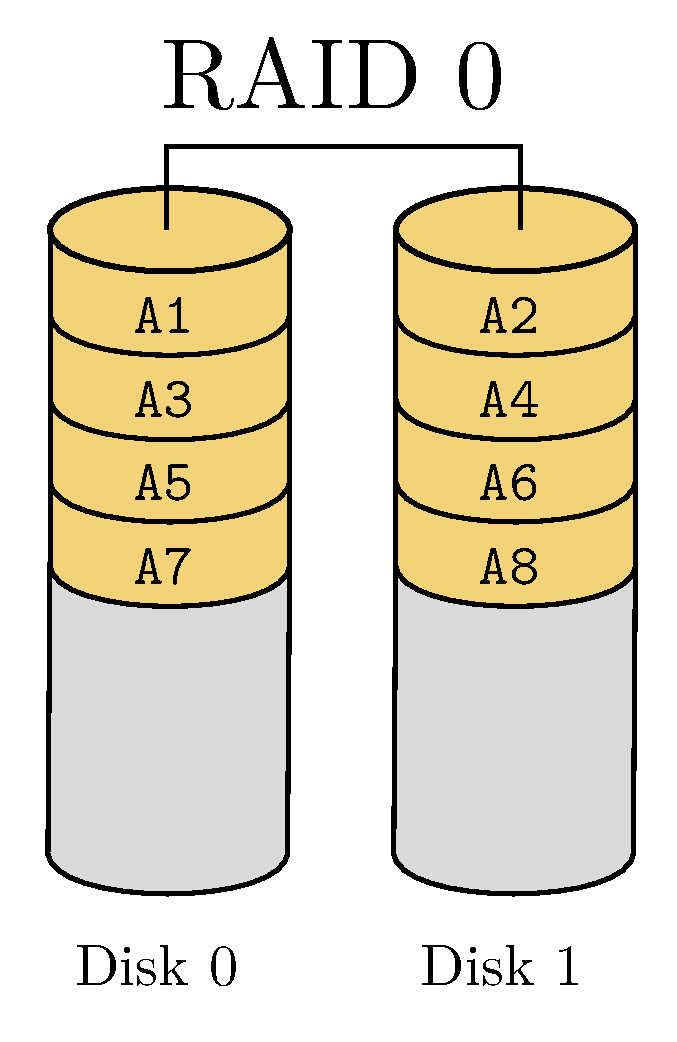
\includegraphics[width=0.25\linewidth]{GrundlagenInfo/05_ErrorChecking/Figures/RAID_0}
    \caption{RAID-0-Architektur mit zwei physischen Festplatten}
    \label{fig:raid0}
\end{figure}

\begin{myexercise}
    Ein System verwendet RAID 0 mit zwei Festplatten, wobei die Daten in 4-Byte-Blöcken verteilt werden. Gegeben ist die folgende Datei:

    \begin{verbatim}
ABCDEFGH
\end{verbatim}

    Wie werden die Daten auf den beiden Festplatten gespeichert?

    \begin{myanswer}
        RAID 0 nutzt Striping ohne Redundanz. Die Daten werden abwechselnd auf die beiden Festplatten geschrieben:

        \begin{verbatim}
Festplatte 1: A C E G
Festplatte 2: B D F H
\end{verbatim}

        Dieses Verfahren erhöht die Geschwindigkeit, bietet jedoch keine Ausfallsicherheit.
    \end{myanswer}
\end{myexercise}

\subsection{RAID 1: Mirroring}
RAID 1 speichert identische Kopien der Daten auf zwei Festplatten (\textit{mirroring}). Fällt eine Festplatte aus, können die Daten von der zweiten Festplatte wiederhergestellt werden.

\begin{itemize}
    \item Vorteil: Sehr hohe Datensicherheit, da jede Information doppelt gespeichert wird.
    \item Nachteil: Speicherplatz wird ineffizient genutzt, da nur die Hälfte der Gesamtkapazität verfügbar ist.
\end{itemize}

\begin{figure}[H]
    \centering
    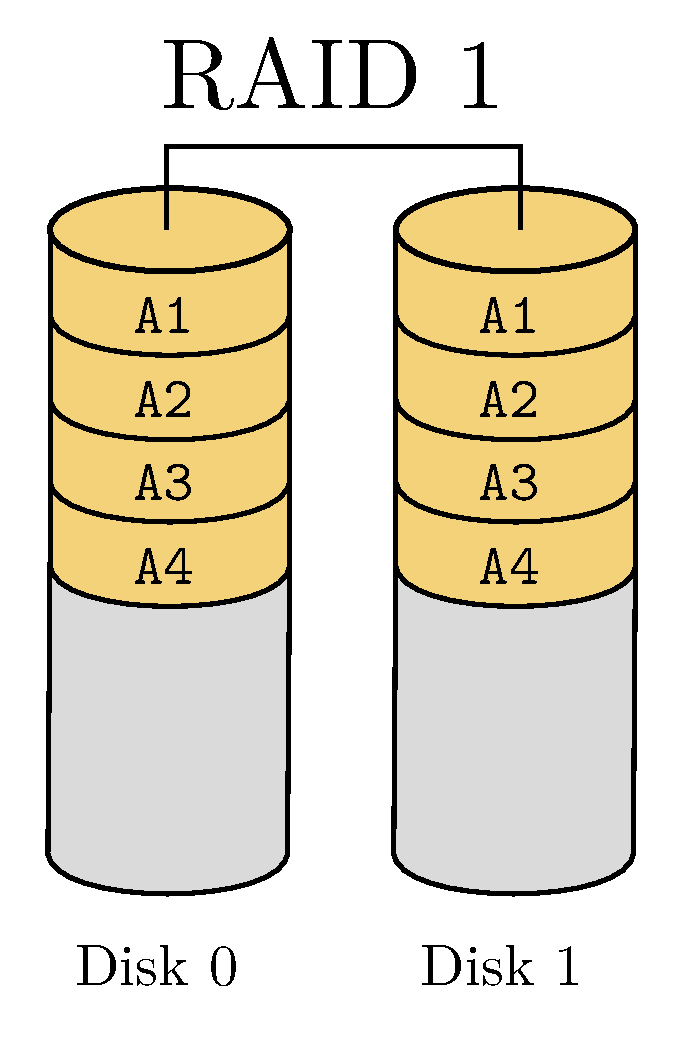
\includegraphics[width=0.25\linewidth]{GrundlagenInfo/05_ErrorChecking/Figures/RAID_1}
    \caption{RAID-1-Architektur mit zwei physischen Festplatten}
    \label{fig:raid1}
\end{figure}

Absicherung gegen Datenverlust kann mit lediglich 2 Festplatten nicht Speicherplatz-effizienter als mit RAID 1 erfolgen, d.h., ein Verlust von 50\% des physischen Speicherplatzes muss in Kauf genommen werden. Effizientere Lösungen bieten sich an, wenn weitere Speicherplatten vorhanden sind. Selbstverständlich kann RAID 1 auch mit 4, 6, 8 oder mehr Festplatten umgesetzt werden.

\begin{myexercise}
    Ein Server verwendet RAID 1 mit zwei Festplatten. Was passiert, wenn eine der beiden Festplatten ausfällt? Kann das System weiterhin genutzt werden?

    \begin{myanswer}
        RAID 1 speichert eine vollständige Kopie aller Daten auf beiden Festplatten (Mirroring). Wenn eine Festplatte ausfällt, kann das System weiterhin auf die zweite Festplatte zugreifen, sodass keine Daten verloren gehen. Die ausgefallene Festplatte sollte jedoch ersetzt werden, um die Redundanz wiederherzustellen.
    \end{myanswer}
\end{myexercise}

\subsection{RAID 4: Paritätsbits}
RAID 4, 5 und 6 nutzen für die Datensicherheit statt \textit{mirroring} (Spiegelung der Daten) einen effizienteren Ansatz, um Daten über mehrere Laufwerke zu verteilen, indem sie Paritätsbits verwenden. Dabei verwendet RAID 5 ein einzelnes Paritätsbit, welches es über verschiedene Festplatten verteilt, so dass jeder ``Striping-Block'' $A_1A_2A_3\cdots$ über genau ein Paritätsbit $A_p$ verfügt (\cref{fig:raid5}).

\begin{figure}[H]
    \centering
    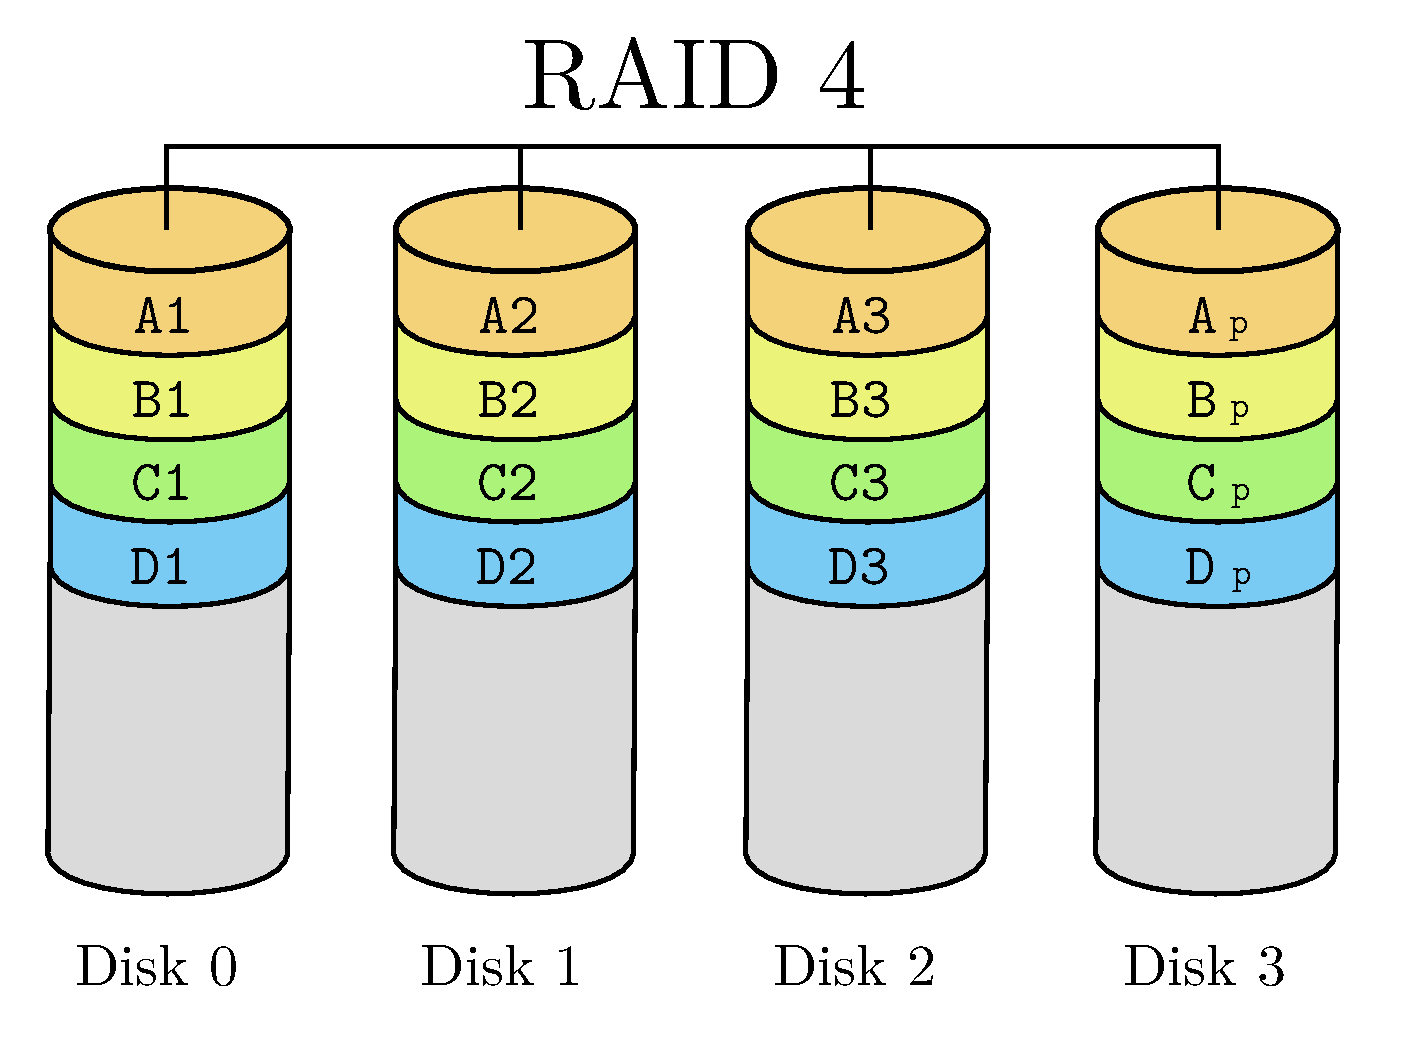
\includegraphics[width=0.45\linewidth]{GrundlagenInfo/05_ErrorChecking/Figures/RAID_4}
    \caption{RAID-4-Architektur mit vier physischen Festplatten und einem Paritätsbit}
    \label{fig:raid4}
\end{figure}

\subsection{RAID 5: Verteilte Paritätsbits}
Da das Paritätsbit bei jedem Schreibvorgang neu geschrieben werden muss (auch bei kleinen Dateien), wird bei RAID-4 die Paritäts-Festplatte übermässig stark beansprucht. Daher werden die Paritätsbits bei RAID-5 im Gegenteil zu RAID-4 auf alle Festplatten verteilt. Ansonsten funktioniert RAID-5 identisch wie RAID-4 (s. \cref{fig:raid5}).


\begin{figure}[H]
    \centering
    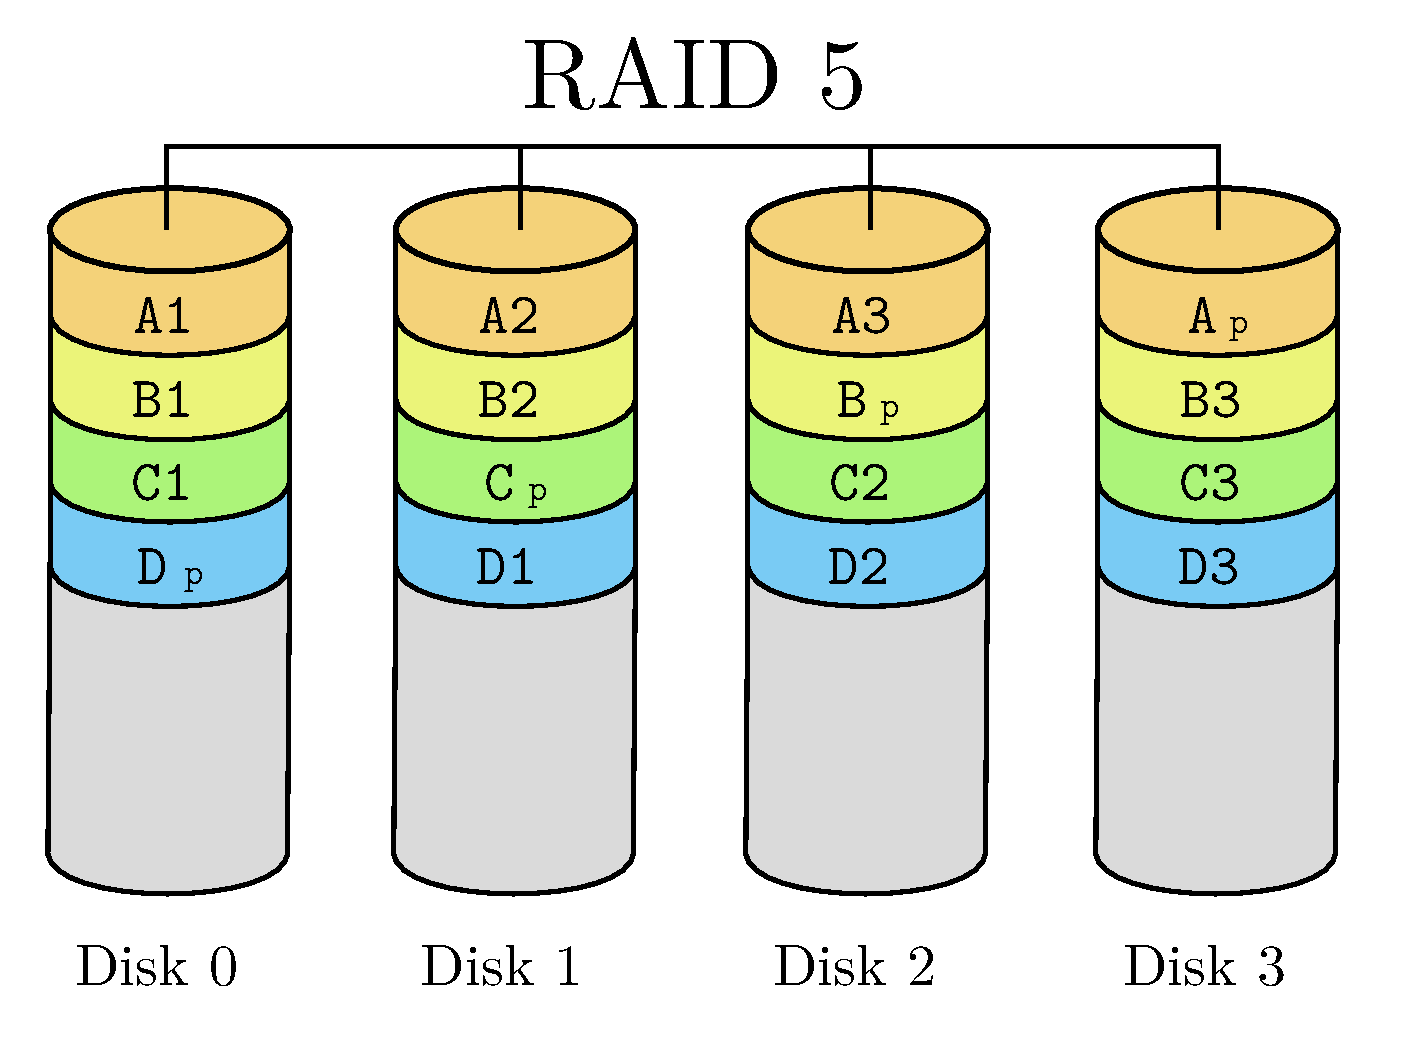
\includegraphics[width=0.45\linewidth]{GrundlagenInfo/05_ErrorChecking/Figures/RAID_5}
    \caption{RAID-5-Architektur mit vier physischen Festplatten und einem \textit{verteilten} Paritätsbit}
    \label{fig:raid5}
\end{figure}


Falls nun eine Festplatte ausfällt, können die verlorengegangenen Daten einfach rekonstruiert werden, indem das \textit{parity bit} über die verbliebenen Datenblöcke erneut berechnet wird. Somit ist ein Speicher-System bei RAID 5 gegen den Ausfall einer Festplatte gesichert.

Bei RAID 5 ist das Paritätsbit für jeden Block auf einer anderen Festplatte gespeichert, wodurch die Performance beim Schreiben von Daten erhöht wird, da die Schreib-Last so auf alle Festplatten gleichmässig verteilt werden kann.

Im Folgenden wird aufgezeigt, wie diese berechnet werden.

RAID 5 verteilt die Paritätsinformationen über alle Festplatten. Die Berechnung erfolgt mit einer XOR-Operation. Beispiel mit vier Datenblöcken $D_1, D_2, D_3, D_4$:

\begin{equation}
    P = D_1 \oplus D_2 \oplus D_3 \oplus D_4
\end{equation}

\begin{myexample}
Nehmen wir an, wir berechnen die Parität für folgende Datenblöcke:
\begin{align*}
    D_1 & = 1101_2 \\
    D_2 & = 1011_2 \\
    D_3 & = 0110_2 \\
    D_4 & = 1001_2
\end{align*}

Die Paritätsberechnung ergibt:
\begin{align*}
    P & = 1101_2 \oplus 1010_2 \oplus 0110_2 \oplus 1001_2 \\
      & = 0001_2
\end{align*}
\end{myexample}

Falls ein Datenblock ausfällt, kann er durch Umstellen der XOR-Operation rekonstruiert werden.

\begin{myexercise}
    Ein RAID-5-System besteht aus drei Festplatten. Die gespeicherten Datenblöcke lauten:

    \begin{align*}
        D_1 & = 1011_2 \\
        D_2 & = 1100_2
    \end{align*}

    Berechne das Paritätsbit $P$ für RAID 5.

    \begin{myanswer}
        Das Paritätsbit wird durch die XOR-Operation berechnet:

        \begin{align*}
            P & = D_1 \oplus D_2       \\
              & = 1011_2 \oplus 1100_2 \\
              & = 0111_2
        \end{align*}

        Das Paritätsbit $P$ wird auf der dritten Festplatte gespeichert, während die Daten auf den ersten beiden Festplatten liegen.
    \end{myanswer}
\end{myexercise}

Je mehr Festplatten verfügbar sind, desto mehr Speicherplatz ist prozentual für die Speicherung von Daten verfügbar. Da immer eine Festplatte für die Datensicherheit verwendet wird, stehen bei 3 Festplatten 2 für die Speicherung von Daten zur Verfügung, bei 4 Festplatten 3, bei 5 Festplatten 4 usw.

\subsection{RAID 6: Zwei Paritätsbits}

Bei RAID-6 werden sogar zwei Paritätsbits verwendet, womit diese Konfiguration Schutz von zwei Festplatten-Ausfällen bietet (\cref{fig:raid6}). Dadurch fallen jedoch auch zwei Festplatten als mögliche Speichermedien weg, da diese für die Datensicherheit benötigt werden.

\begin{figure}[H]
    \centering
    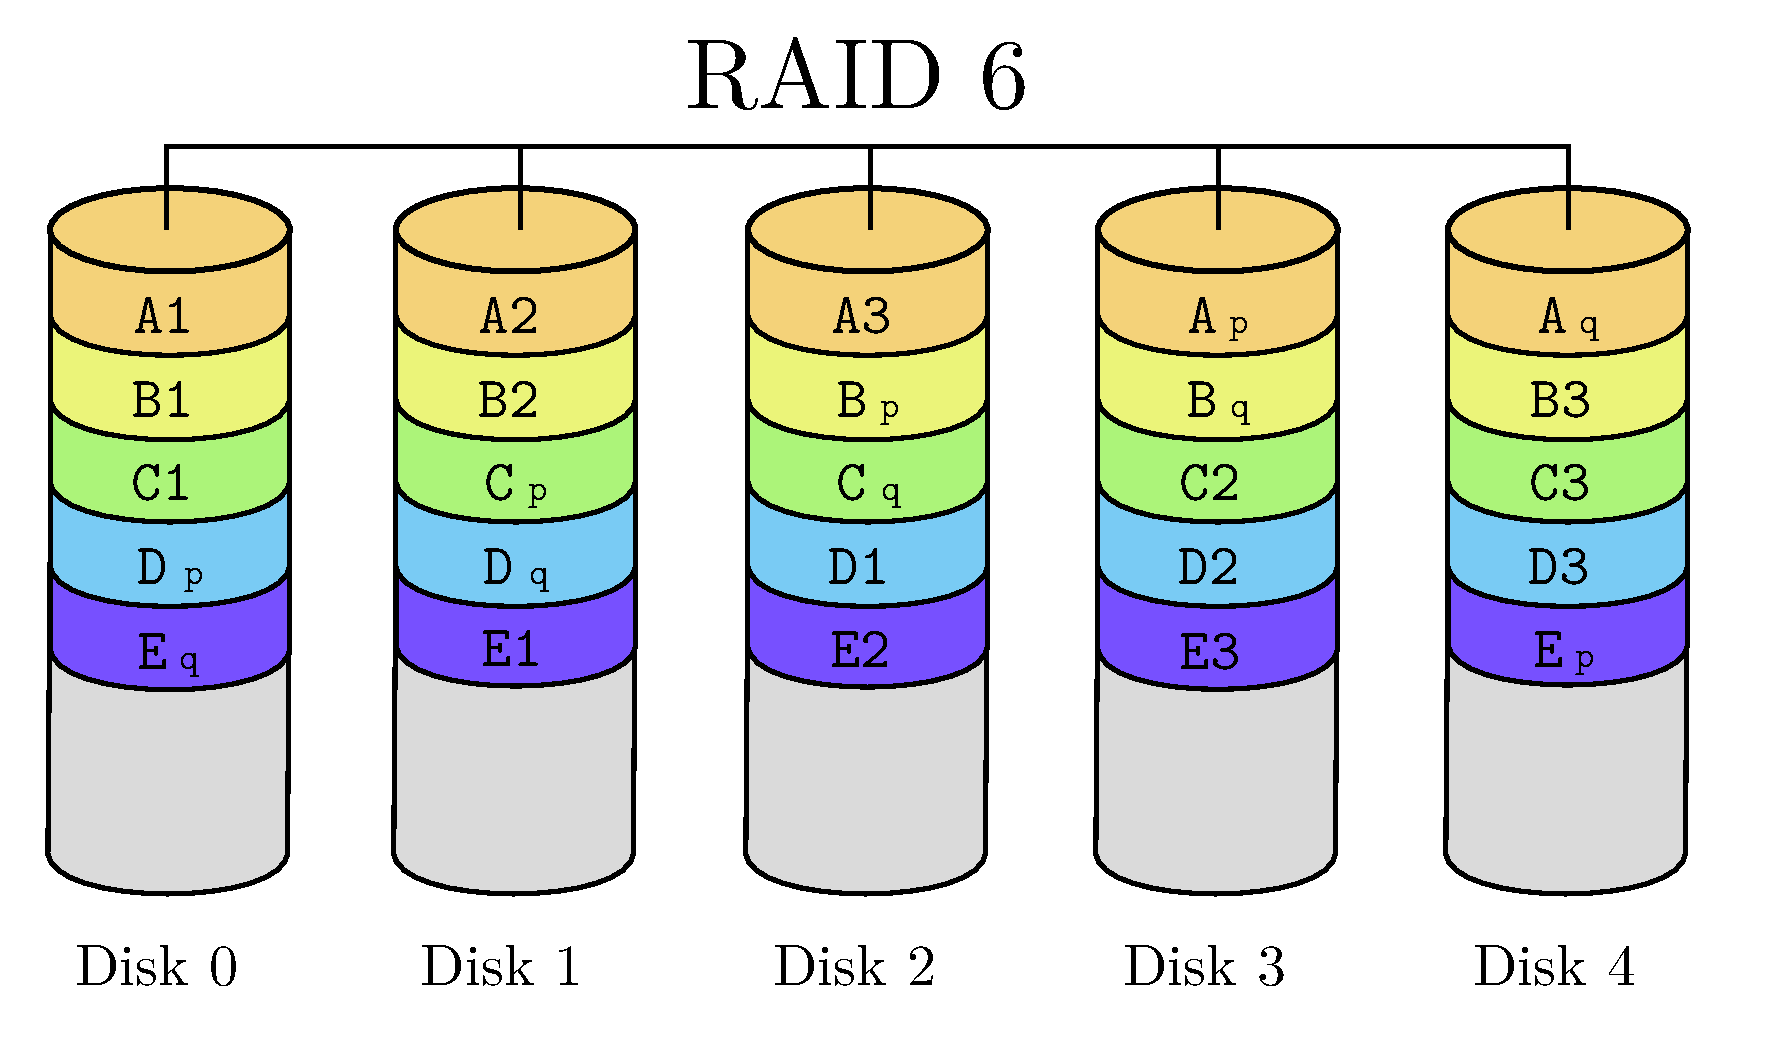
\includegraphics[width=0.5\linewidth]{GrundlagenInfo/05_ErrorChecking/Figures/RAID_6}
    \caption{RAID 5-Architektur mit fünf physischen Festplatten und zwei Paritätsbits}
    \label{fig:raid6}
\end{figure}

RAID 6 verwendet zwei Paritätswerte: eine XOR-basierte Parität ($P$) wie in RAID 5 und eine zweite Parität $Q$, die durch eine Galois-Feld-Multiplikation berechnet wird. Für Beispiele einer Berechnung des zweiten Paritätsbits sei auf die Webseite von \href{https://blogs.oracle.com/solaris/post/understanding-raid-6-with-junior-high-math}{Oracle} hingewiesen.

\begin{myexercise}
    Marina gründet eine IT-Firma und kauft sich 8 Festplatten für die Speicherung ihrer Daten. Da sie viele Daten hat, möchte sie möglichst viel nutzbaren Speicherplatz haben, gleichzeitig möchte sie gegen den Ausfall von \textit{einer} Festplatte geschützt sein. Welche RAID-Konfiguration empfehlen Sie Marina (0, 1, 5 oder 6)? Begründen Sie Ihre Antwort.
    \begin{myanswer}
        \begin{itemize}
            \item \textbf{Empfohlen: RAID 5} – Maximiert Speicherplatz, schützt vor \textbf{1 Festplatten-Ausfall}.
            \item \textbf{Speicherausnutzung:} 7 von 8 Platten für Daten, 1 für Parität.
            \item \textbf{Performance:} Gutes \textbf{Lesen}, etwas langsameres \textbf{Schreiben} (Paritätsberechnung).
            \item \textbf{Alternative: RAID 6} – Mehr Sicherheit (\textbf{2 Plattenausfälle möglich}), aber weniger Speicher (6 nutzbar).
        \end{itemize}
    \end{myanswer}


\end{myexercise}

\begin{myexercise}
    Lara möchte ihre schönsten Fotos sichern und hat sich dazu zwei Festplatten gekauft. Da ihre Fotos für sie wichtig sind, möchte sie sich gegen den Ausfall einer Festplatte schützen und entscheidet sich daher für eine RAID-1-Konfiguration.

    \begin{itemize}
        \item Weshalb kann Lara selbst dann, wenn sie sich zwei gleich grosse Festplatten kauft, nur maximal die Hälfte des Speicherplatzes für sich nutzen?
        \item Welche alternative RAID-Konfiguration könnte Lara in Betracht ziehen, um mehr Speicherplatz zu erhalten? Was wären Nachteile davon?
        \item Welche RAID-Alternative gäbe es für Lara, um sowohl mehr Speicher als auch Redundanz zu gewährleisten?
    \end{itemize}


    \begin{myanswer}
        \begin{itemize}
            \item \textbf{RAID 1}: Speicherhalbierung, da alle Daten gespiegelt werden (\textbf{mirroring}, redundante Kopie).
            \item \textbf{Alternative}: RAID 0 (\textbf{striping}) $\rightarrow$ \textbf{doppelter Speicherplatz}, aber \textbf{kein Schutz} bei Festplattenausfall.
            \item \textbf{Kompromiss}: RAID 5 (mind. 3 Platten) $\rightarrow$ \textbf{mehr Speicher} als RAID 1, aber trotzdem \textbf{Redundanz}.
        \end{itemize}
    \end{myanswer}
\end{myexercise}

\begin{myexercise}
    Bestimmen Sie für den Fall, dass sie 6 Festplatten gleicher Grösse besitzen, den verfügbaren Speicherplatz für die Konfigurationen RAID 0, RAID 1, RAID 4, RAID 5 und RAID 6. Geben Sie den verfügbaren Speicherplatz als Bruch an (z.B. 3/6). Geben Sie zudem die Ausfallsicherheit an (wie viele Festplatten können ausfallen ohne Datenverlust?).

    \begin{table}[H]
        \centering
        \begin{tabular}{c||c|c}
            \textbf{Konfiguration} & \textbf{Verfügbare Festplatten} & \textbf{Ausfallsicherheit} \\\midrule\midrule
            \textbf{RAID 0}        &                                 &                            \\[1cm]\midrule
            \textbf{RAID 1}        &                                 &                            \\[1cm]\midrule
            \textbf{RAID 4}        &                                 &                            \\[1cm]\midrule
            \textbf{RAID 5}        &                                 &                            \\[1cm]\midrule
            \textbf{RAID 6}        &                                 &                            \\[1cm]
        \end{tabular}
    \end{table}
    \begin{myanswer}
        \begin{table}[H]
            \centering
            \begin{tabular}{c||c|c}
                \textbf{Konfiguration} & \textbf{Verfügbare Festplatten} & \textbf{Ausfallsicherheit} \\\midrule\midrule
                \textbf{RAID 0}        & 6/6                             & 0                          \\\midrule
                \textbf{RAID 1}        & 3/6                             & 1                          \\\midrule
                \textbf{RAID 5}        & 5/6                             & 1                          \\\midrule
                \textbf{RAID 6}        & 4/6                             & 2                          \\
            \end{tabular}
        \end{table}
    \end{myanswer}
\end{myexercise}


